%% abtex2-modelo-trabalho-academico.tex, v-1.9.2 laurocesar
%% Copyright 2012-2014 by abnTeX2 group at http://abntex2.googlecode.com/ 
%%
%% This work may be distributed and/or modified under the
%% conditions of the LaTeX Project Public License, either version 1.3
%% of this license or (at your option) any later version.
%% The latest version of this license is in
%%   http://www.latex-project.org/lppl.txt
%% and version 1.3 or later is part of all distributions of LaTeX
%% version 2005/12/01 or later.
%%
%% This work has the LPPL maintenance status `maintained'.
%% 
%% The Current Maintainer of this work is the abnTeX2 team, led
%% by Lauro César Araujo. Further information are available on 
%% http://abntex2.googlecode.com/
%%
%% This work consists of the files abntex2-modelo-trabalho-academico.tex,
%% abntex2-modelo-include-comandos and abntex2-modelo-references.bib
%%

% ------------------------------------------------------------------------
% ------------------------------------------------------------------------
% abnTeX2: Modelo de Trabalho Academico (tese de doutorado, dissertacao de
% mestrado e trabalhos monograficos em geral) em conformidade com 
% ABNT NBR 14724:2011: Informacao e documentacao - Trabalhos academicos -
% Apresentacao
% ------------------------------------------------------------------------
% ------------------------------------------------------------------------

\documentclass[
	% -- opções da classe memoir --
	12pt,				% tamanho da fonte
	openright,			% capítulos começam em pág ímpar (insere página vazia caso preciso)
	twoside,			% para impressão em verso e anverso. Oposto a oneside
	a4paper,			% tamanho do papel. 
	% -- opções da classe abntex2 --
	%chapter=TITLE,		% títulos de capítulos convertidos em letras maiúsculas
	%section=TITLE,		% títulos de seções convertidos em letras maiúsculas
	%subsection=TITLE,	% títulos de subseções convertidos em letras maiúsculas
	%subsubsection=TITLE,% títulos de subsubseções convertidos em letras maiúsculas
	% -- opções do pacote babel --
	english,			% idioma adicional para hifenização
	french,				% idioma adicional para hifenização
	spanish,			% idioma adicional para hifenização
	brazil				% o último idioma é o principal do documento
	]{abntex2}

% ---
% Pacotes básicos 
% ---
\usepackage{lmodern}			% Usa a fonte Latin Modern			
\usepackage[T1]{fontenc}		% Selecao de codigos de fonte.
\usepackage[utf8]{inputenc}		% Codificacao do documento (conversão automática dos acentos)
\usepackage{lastpage}			% Usado pela Ficha catalográfica
\usepackage{indentfirst}		% Indenta o primeiro parágrafo de cada seção.
\usepackage{color}				% Controle das cores
\usepackage{graphicx}			% Inclusão de gráficos
\usepackage{microtype} 			% para melhorias de justificação
\usepackage{pythonhighlight}
\usepackage{listings}
\usepackage{xcolor}
\usepackage{bm}
% ---
		
% ---
% Pacotes adicionais, usados apenas no âmbito do Modelo Canônico do abnteX2
% ---
\usepackage{lipsum}				% para geração de dummy text
\usepackage{tabularx}
% ---

% ---
% Pacotes de citações
% ---
\usepackage[brazilian,hyperpageref]{backref}	 % Paginas com as citações na bibl
\usepackage[alf]{abntex2cite}	% Citações padrão ABNT

% --- 
% CONFIGURAÇÕES DE PACOTES
% --- 
\lstset{
  basicstyle=\fontsize{11}{13}\selectfont\ttfamily
}
\graphicspath{ {./images/} }
% ---
% Configurações do pacote backref
% Usado sem a opção hyperpageref de backref
\renewcommand{\backrefpagesname}{Citado na(s) página(s):~}
% Texto padrão antes do número das páginas
\renewcommand{\backref}{}
% Define os textos da citação
\renewcommand*{\backrefalt}[4]{
	\ifcase #1 %
		Nenhuma citação no texto.%
	\or
		Citado na página #2.%
	\else
		Citado #1 vezes nas páginas #2.%
	\fi}%
% ---

% ---
% Informações de dados para CAPA e FOLHA DE ROSTO
% ---
\titulo{Relatório}
\autor{Bruno Duarte Barreto Borges\\Fabio Oliveira de Abreu\\Erik Kazuo Sugawara}
\local{Florianópolis, SC}
\data{2021}
\orientador{Alvaro Junio Pereira Franco}
\instituicao{%
  Universidade Federal de Santa Catarina
  \par
  Departamento de Informática e Estatística
  \par
  INE5426 - Construção de Compiladores}
\tipotrabalho{Relatório}
% O preambulo deve conter o tipo do trabalho, o objetivo, 
% o nome da instituição e a área de concentração 
\preambulo{Relatório sobre a Construção de um Compilador, feito 
pelos alunos: Bruno Duarte Barreto Borges, Fabio Oliveira de Abreu e
Erik Kazuo Sugawara. Para obtenção da aprovação na disciplina Construção
de Compiladores, ministrada pelo Prof. Dr. Alvaro Junio Pereira Franco.}
% ---


% ---
% Configurações de aparência do PDF final

% alterando o aspecto da cor azul
\definecolor{blue}{RGB}{41,5,195}

% informações do PDF
\makeatletter
\hypersetup{
     	%pagebackref=true,
		pdftitle={\@title}, 
		pdfauthor={\@author},
    	pdfsubject={\imprimirpreambulo},
	    pdfcreator={LaTeX with abnTeX2},
		pdfkeywords={abnt}{latex}{abntex}{abntex2}{trabalho acadêmico}, 
		colorlinks=true,       		% false: boxed links; true: colored links
    	linkcolor=blue,          	% color of internal links
    	citecolor=blue,        		% color of links to bibliography
    	filecolor=magenta,      		% color of file links
		urlcolor=blue,
		bookmarksdepth=4
}
\makeatother
% --- 

% --- 
% Espaçamentos entre linhas e parágrafos 
% --- 

% O tamanho do parágrafo é dado por:
\setlength{\parindent}{1.3cm}

% Controle do espaçamento entre um parágrafo e outro:
\setlength{\parskip}{0.2cm}  % tente também \onelineskip

% ---
% compila o indice
% ---
\makeindex
% ---

% ----
% Início do documento
% ----
\begin{document}

% Retira espaço extra obsoleto entre as frases.
\frenchspacing 

% ----------------------------------------------------------
% ELEMENTOS PRÉ-TEXTUAIS
% ----------------------------------------------------------
% \pretextual

% ---
% Capa
% ---
\imprimircapa
% ---

% ---
% Folha de rosto
% (o * indica que haverá a ficha bibliográfica)
% ---
\imprimirfolhaderosto*
% ---

% ---
% Inserir a ficha bibliografica
% ---

% Isto é um exemplo de Ficha Catalográfica, ou ``Dados internacionais de
% catalogação-na-publicação''. Você pode utilizar este modelo como referência. 
% Porém, provavelmente a biblioteca da sua universidade lhe fornecerá um PDF
% com a ficha catalográfica definitiva após a defesa do trabalho. Quando estiver
% com o documento, salve-o como PDF no diretório do seu projeto e substitua todo
% o conteúdo de implementação deste arquivo pelo comando abaixo:
%
% \begin{fichacatalografica}
%     \includepdf{fig_ficha_catalografica.pdf}
% \end{fichacatalografica}

% ---
% inserir lista de abreviaturas e siglas
% ---
\begin{siglas}
  \item[PLY] Python Lexx-Yacc
  \item[BNF] Bakus-Naur Form
  \item[Yacc] Yet Another Compiler-Compiler
\end{siglas}
% ---

% ---
% inserir o sumario
% ---
\pdfbookmark[0]{\contentsname}{toc}
\tableofcontents*
\cleardoublepage
% ---



% ----------------------------------------------------------
% ELEMENTOS TEXTUAIS
% ----------------------------------------------------------
\textual

% ----------------------------------------------------------
% Introdução (exemplo de capítulo sem numeração, mas presente no Sumário)
% ----------------------------------------------------------
\chapter*[Introdução]{Introdução}
\addcontentsline{toc}{chapter}{Introdução}
% ----------------------------------------------------------

Um compilador é um programa de sistema que traduz uma linguagem de alto nível
para um programa equivalente em código de máquina para um processador. Sendo assim,
um compilador não produz diretamente o código de máquina, mas sim um programa
semanticamente equivalente na linguagem simbólica (assembly), que é traduzido para o programa em linguagem de máquina através de montadores\footnote{\url{https://www.dca.fee.unicamp.br/cursos/EA876/apostila/HTML/node37.html}}.

Este trabalho, em sua primeira fase, tem como objetivo criar um compilador através de um
analisador léxico e sintático para uma linguagem (AL). Para facilitar os estudos na criação do compilador,
foi disponibilizada a linguagem ``LCC-2021-2'' derivada da gramática ``CC-2021-2''
na forma BNF(Backus-Naur Form), inspirada na gramática X++ de Delamaro
\footnote{\url{http://conteudo.icmc.usp.br/pessoas/delamaro/SlidesCompiladores/
CompiladoresFinal.pdf}}. Na sua segunda parte, iremos modificar a gramática
de forma que ela seja coerente para o analisador sintático e o código analisado
deve ser aceito por ele.

As atividades contidas neste relatório foram feitas com a linguagem Python em
conjunto da ferramenta PLY (Python Lex-Yacc)\footnote{\url{https://www.dabeaz.com/ply/}},
uma implementação dos geradores de analisadores léxico e sintático (Lex-Yacc) para Python.
Dessa forma, com o auxílio de ferramentas que permitem gerar analisadores, mostraremos
o funcionamento do analisador léxico através de seu algoritmo e da sua aplicação com 
exemplos de programas em alto nível baseadas na gramática ``CC-2021-2''.




% ----------------------------------------------------------
% PARTE
% ----------------------------------------------------------
\part{Ferramenta}
% ----------------------------------------------------------
\chapter{Python Lex-Yacc}
\section{Sobre a ferramenta}
O PLY é uma implementação pura em Python baseada nas ferramentas de construção
de compiladores lex e yacc. Possui suporte para LARL(1) e mecanismos
de validação, verificação de erros e diagnósticos. Sua primeira versão foi desenvolvida
na Universidade de Chicago, para dar suporte à disciplina Introdução a Compiladores.
A sua versão mais recente é o PLY-4.0, que requer o Python na versão 3.6 ou mais nova. 

Ele consiste em dois módulos separados: o lex.py e o yacc.py. O módulo lex.py é utilizado
para separar as entradas em texto do código em uma coleção de tokens baseadas em suas respectivas 
expressões regulares. O yacc.py é utilizado para reconhecer a sintaxe de uma linguagem 
baseada em uma gramática livre de contexto. Além disso, possui utilidades como verificação
de erros, validação de gramática, suporte para produções vazias, tokens de erros e regras de
precedência para resolver ambiguidades.

\section{Lex}
O Lex é utilizado para realizar a atribuição dos tokens com as entradas (\emph{strings}).
Os nomes dos tokens podem ser declarados de forma simples através de uma lista. Um token
que é identificado se torna um objeto da classe LexToken.
\begin{python}
import ply.lex as lex
import ply.yacc as yacc

# RESERVED WORDS
reserved = [
    'DEF',         # def
    'BREAK',       # break
    'FOR',         # for
    'IF',          # if
    'ELSE',        # else
    'INT',         # int
    'FLOAT',       # float
    'NEW',         # new
    'PRINT',       # print
    'READ',        # read
    'RETURN',      # return
    'STRING',      # string
]
\end{python}

	Dada uma lista de tokens, podemos definir suas expressões regulares, que podem
ser de forma simples ou complexa. Note que por definição da ferramenta,
as expressões regulares são declaradas como uma variável que se inicia com ``t\_'',
seguida pelo nome do token definido na lista. Segue um exemplo das expressões
regulares para tokens simples, como: \emph{Assign, Greater Than, Less Than, Equals, Less Equal,
Greater Equal, Not Equal, Plus, Minus, Multiply, Divide e Rem}.
\\
\begin{python}
t_ASSIGN = r'\='
t_GT = r'\>'
t_LT = r'\<'
t_EQ = r'\=='
t_LE = r'\<='
t_GE = r'\>='
t_NEQ = r'\!='
t_PLUS = r'\+'
t_MINUS = r'\-'
t_MULTIPLY = r'\*'
t_DIVIDE = r'\/'
t_REM = r'\%'
\end{python}

Para tokens que requerem maior complexidade para serem identificados, podemos declará-los através de funções
que também se iniciam pelos caracteres ``t\_'' seguidos pelo nome do token
definido. Note que também podemos realizar o tratamento dos valores obtidos acessando
o atributo \emph{value} do objeto LexToken.
\\
\begin{python}
def t_float_constant(t):
    r'[+-]?\d+\.\d+([eE][+-]?\d+)?'
    t.value = float(t.value)
    return t

def t_int_constant(t):
    r'[+-]?\d+'
    t.value = int(t.value)
    return t

def t_string_constant(t):
    r'"[^"\n\r]*"'
    return t

def t_IDENT(t):
    r'[a-zA-Z_][a-zA-Z_0-9]*'
    return t
\end{python}
\newpage


Com essa ferramenta também podemos fazer tratativas de leitura e identificação de erros.
Ela também segue as definições de nomenclatura para tokens. Seguem alguns exemplos
de tratamento de leitura para ignorar caracteres em branco, fim de linhas e caracteres ilegais.
\begin{python}
t_ignore = r' ' # Ignore spaces between char.

def t_newline(t):
	r'\n+'
	t.lexer.lineno += len(t.value)

def t_error(t):
    errors.append("Illegal char %s in line %d, column %d" % (t.value[0], t.lexer.lineno, find_column(t)))
    t.lexer.skip(1)

\end{python}

Para demonstrar o funcionamento do analisador léxico, executamos o seguinte
código. A saída é um LexToken, onde os atributos correspondem respectivamente ao 
identificador do token, símbolo, linha e coluna.

\begin{python}
# Test it out
data = '''
3 + 4 * 10
'''

# Give the lexer some input
lexer.input(data)

# Tokenize
while True:
    tok = lexer.token()
    if not tok:
        break      # No more input
    print(tok)
\end{python}
\noindent Saída :
\begin{lstlisting}[language=bash]
    LexToken(NUMBER,3,2,1)
    LexToken(PLUS,'+',2,3)
    LexToken(NUMBER,4,2,5)
    LexToken(MULTIPLY,'*',2,7)
    LexToken(NUMBER,10,2,10)

\end{lstlisting}
% ---
% Capitulo com exemplos de comandos inseridos de arquivo externo 
% ---
\include{abntex2-modelo-include-comandos}
% ---

% ----------------------------------------------------------
% PARTE
% ----------------------------------------------------------
\part{Analisador Léxico}
% ----------------------------------------------------------

% ---
% Capitulo de revisão de literatura
% ---
\chapter{Metodologia}
% ---

% ---
\section{Extração dos tokens}
% ---
	Para obter os tokens, utilizamos a gramática ``CC-2021-2'' como base
    e dividimos cada um deles em um dos seguintes grupos: palavras reservadas,
	operadores, símbolos especiais, constantes e identificadores. Além disso,
	alteramos a gramática de modo que seja possível retornar valores com o token ``\emph{return}''.

\begin{python}
# RESERVED WORDS
reserved = [
    'DEF',         # def
    'BREAK',       # break
    'FOR',         # for
    'IF',          # if
    'ELSE',        # else
    'INT',         # int
    'FLOAT',       # float
    'NEW',         # new
    'PRINT',       # print
    'READ',        # read
    'RETURN',      # return
    'STRING',      # string
] 
\end{python}

\begin{python}
# OPERATORS
operators = [
    'ASSIGN',      # =
    'GT',          # >
    'LT',          # <
    'EQ',          # ==
    'LE',          # <=
    'GE',          # >=
    'NEQ',         # !=
    'PLUS',        # +
    'MINUS',       # -
    'MULTIPLY',    # *
    'DIVIDE',      # / 
    'REM'          # %
]
\end{python}
\newpage

\begin{python}
# SPECIAL SYMBOLS
special = [
    'LPAREN',      # (
    'RPAREN',      # )
    'LBRACE',      # {
    'RBRACE',      # }
    'LBRACKET',    # [
    'RBRACKET',    # ]
    'SEMICOLON',   # ;
    'COMMA',       # ,
]
\end{python}

\begin{python}
# CONSTANTS
constant = [
    'int_constant',
    'string_constant',
    'float_constant',
    'null_constant'
]
\end{python}

\begin{python}
# IDENTIFIERS
identifiers = [
    'IDENT'
]
\end{python}

\begin{python}
tokens = reserved + operators + special + constant + identifiers
\end{python}
\section{Expressões Regulares}
Após a identificação dos tokens, criamos a expressão regular de cada um deles.
\begin{python}
t_ignore = r' ' # Ignore spaces between char.

def t_DEF(t):
    r'def'
    return t

def t_BREAK(t):
    r'break'
    return t

def t_FOR(t):
    r'for'
    return t
\end{python}

\begin{python}
def t_IF(t):
    r'if'
    return t

def t_ELSE(t):
    r'else'
    return t

def t_NEW(t):
    r'new'
    return t

def t_PRINT(t):
    r'print'
    return t

def t_READ(t):
    r'read'
    return t

def t_RETURN(t):
    r'return'
    return t

def t_STRING(t):
    r'string'
    return t

def t_INT(t):
    r'int'
    return t

def t_FLOAT(t):
    r'float'
    return t
\end{python}

\begin{python}
def t_null_constant(t):
    r'null'
    return t

def t_float_constant(t):
    r'[+-]?\d+\.\d+([eE][+-]?\d+)?'
    t.value = float(t.value)
    return t
\end{python}
\newpage
\begin{python}
def t_int_constant(t):
    r'[+-]?\d+'
    t.value = int(t.value)
    return t

def t_string_constant(t):
    r'"[^"\n\r]*"'
    return t

def t_IDENT(t):
    r'[a-zA-Z_][a-zA-Z_0-9]*'
    return t

def t_newline(t):
    r'\n+'
    t.lexer.lineno += len(t.value)

errors = []

def t_error(t):
    errors.append("Illegal char %s in line %d, column %d" % (t.value[0], t.lexer.lineno, find_column(t)))
    t.lexer.skip(1)
\end{python}

Além da criação das expressões regulares, também foi criado uma função que imprime 
a tabela de símbolos de forma elegante no terminal.
\\
\begin{python}
def print_table(lexer):
    pattern = "{:^25} | {:^60} | {:^7} | {:^7}"
    print("\033[4m" + pattern.format("TOKEN", "VALUE", "LINE", "COLUMN") + "\033[0m")
    while True:
        tok = lexer.token()
        if not tok:
            break
        print(pattern.format(tok.type, tok.value, tok.lineno, find_column(tok))) 

    for e in errors:
        print(e)

\end{python}
\newpage
\section{Analisador Léxico}
Com os tokens e expressões regulares definidos, executamos o analisador léxico e obtemos
a sua tabela de símbolos formatada através da função ``print\_table''.

\begin{lstlisting}[language=bash]
		$ make run file='tmp/lil_example.lcc'

             TOKEN      |    VALUE    |  LINE   | COLUMN 
              DEF       |     def     |    1    |    1   
             IDENT      | hello_world |    1    |    5   
            LPAREN      |      (      |    1    |   16   
            RPAREN      |      )      |    1    |   17   
            LBRACE      |      {      |    1    |   19   
             PRINT      |    print    |    2    |    5   
        string_constant |"hello world"|    2    |   11   
           SEMICOLON    |      ;      |    2    |   24   
            RBRACE      |      }      |    3    |    1   
              INT       |     int     |    5    |    1   
             IDENT      |      x      |    5    |    5   
           SEMICOLON    |      ;      |    5    |    6   
             IDENT      |      x      |    6    |    1   
            ASSIGN      |      =      |    6    |    3   
         int_constant   |      10     |    6    |    5   
           SEMICOLON    |      ;      |    6    |    7   
              IF        |      if     |    8    |    1   
            LPAREN      |      (      |    8    |    4   
             IDENT      |      x      |    8    |    5   
              GT        |      >      |    8    |    7   
         int_constant   |      30     |    8    |    9   
            RPAREN      |      )      |    8    |   11   
            LBRACE      |      {      |    8    |   13   
             IDENT      | hello_world |    9    |    5   
            LPAREN      |      (      |    9    |   16   
            RPAREN      |      )      |    9    |   17   
           SEMICOLON    |      ;      |    9    |   18   
            RBRACE      |      }      |   10    |    1   
             ELSE       |     else    |   10    |    3   
            LBRACE      |      {      |   10    |    8   
             PRINT      |    print    |   11    |    5   
        string_constant |    "erro"   |   11    |   11   
           SEMICOLON    |      ;      |   11    |   17   
            RBRACE      |      }      |   12    |    1  
\end{lstlisting}


% ----------------------------------------------------------
% PARTE
% ----------------------------------------------------------
% ----------------------------------------------------------

% ---
% primeiro capitulo de Resultados
% ---
\chapter{Diagrama de Transição}
% ---
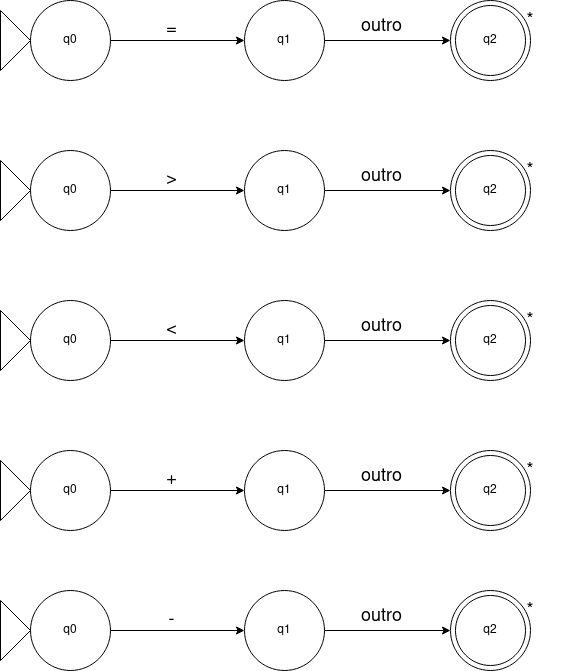
\includegraphics[scale=0.7]{1.png}
\\
\\
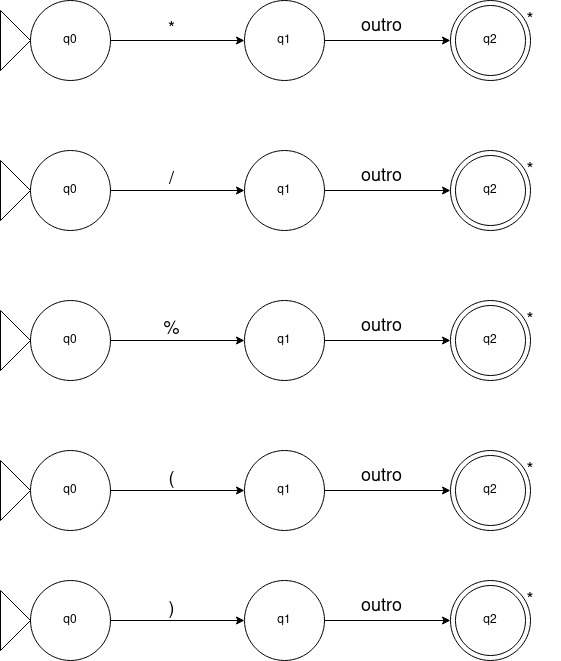
\includegraphics[scale=0.7]{2.png}
\\
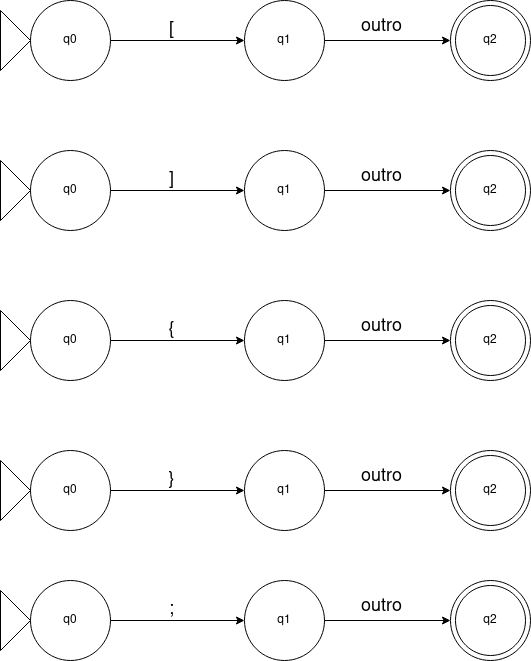
\includegraphics[scale=0.7]{3.png}
\\
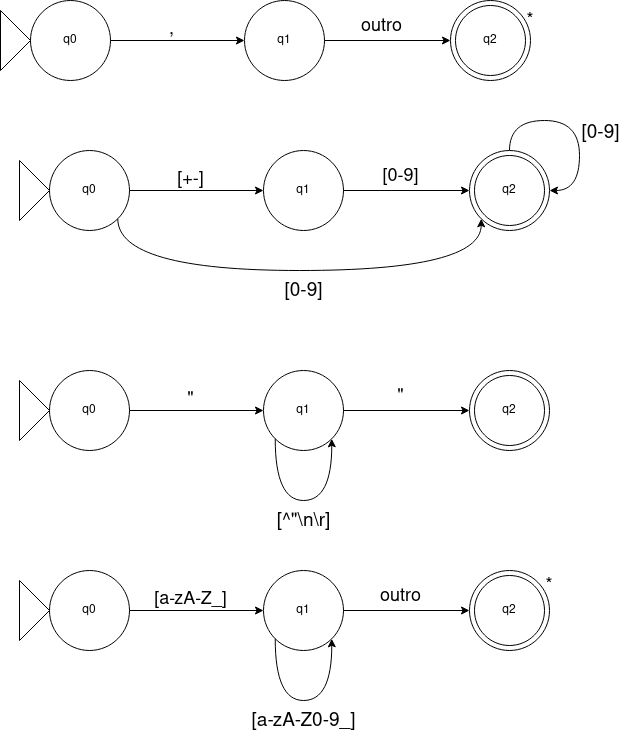
\includegraphics[scale=0.7]{4.png}
\\
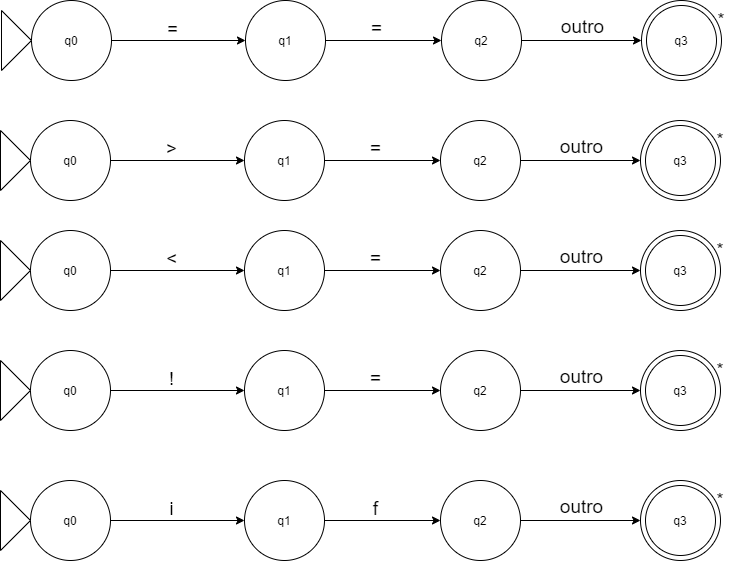
\includegraphics[scale=0.7]{5.png}
\\
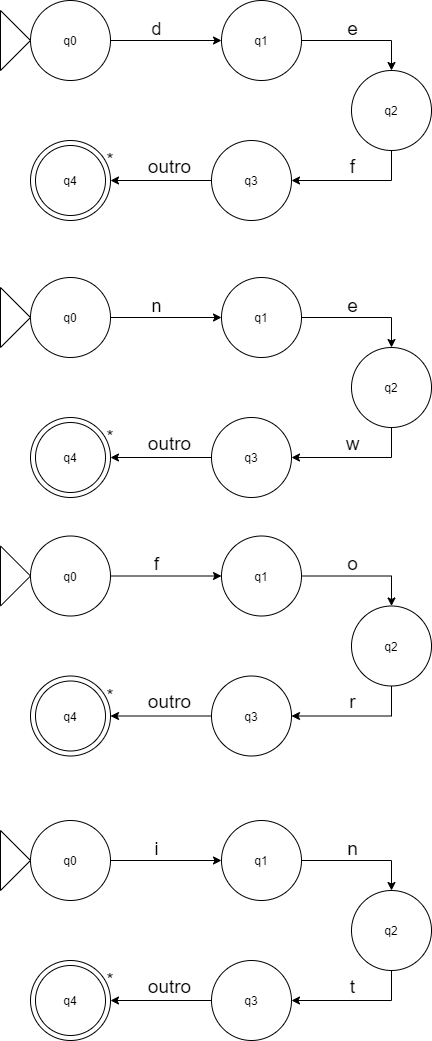
\includegraphics[scale=0.7]{6.png}
\\
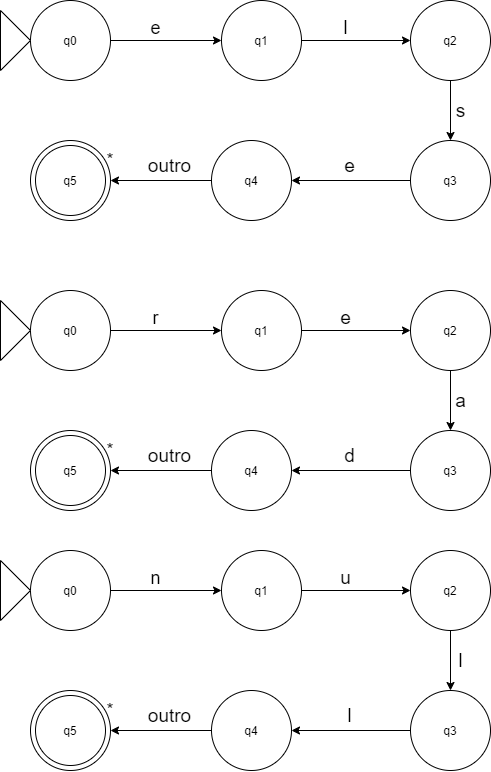
\includegraphics[scale=0.7]{7.png}
\\
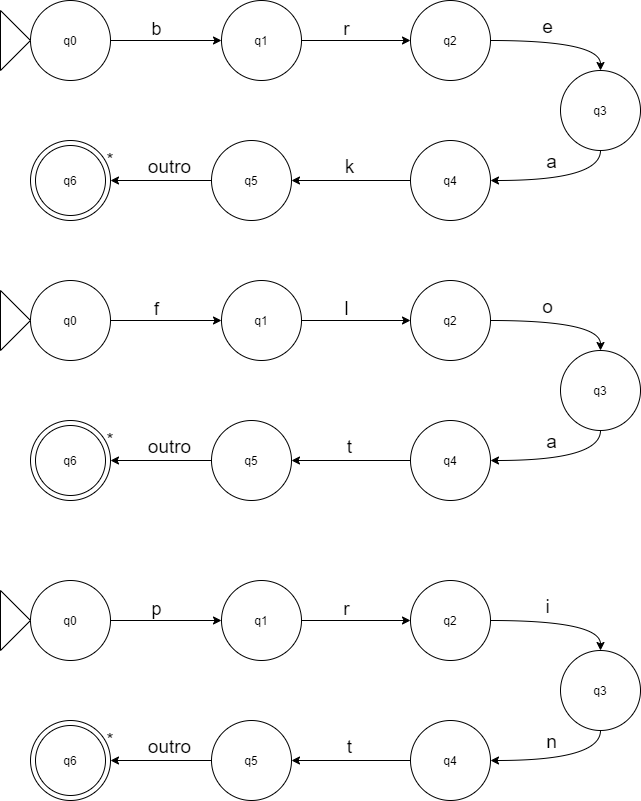
\includegraphics[scale=0.7]{8.png}
\\
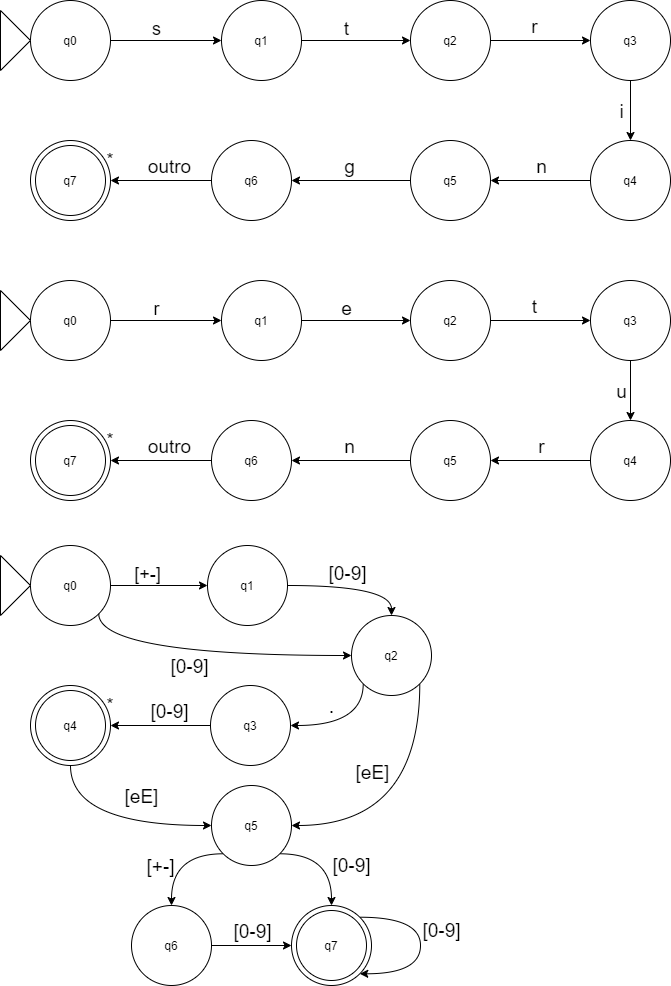
\includegraphics[scale=0.7]{9.png}

% ----------------------------------------------------------
% Finaliza a parte no bookmark do PDF
% para que se inicie o bookmark na raiz
% e adiciona espaço de parte no Sumário
% ----------------------------------------------------------
\phantompart
\part{Analisador Sintático}
\chapter{Ferramenta}
\section{Yacc}
O Yacc é uma abreviação do termo em inglês "\emph{Yet Another Compiler-Compiler}",
semelhante a ferramenta de mesmo nome para Unix. Ele é o componente do PLY que realiza
a análise da gramática.

Cada regra gramatical pode ser definida atravé de uma função Python, onde cada \emph{docstring} possui
a especificação apropriada da gramática livre de contexto. Cada função aceita um
único argumento `\textbf{p}', que é a sequência contendo os valores de cada símbolo da gramática
da respectiva regra. Segue um exemplo, de como especificamos a regra para a expressão \textbf{FUNCDEF}.

\begin{python}
def p_funcdef(p):
    '''
    funcdef : DEF IDENT LPAREN paramlist RPAREN LBRACE statelist RBRACE
    '''
\end{python}

Normalmente, a primeira regra especificada no yacc determina o começo da gramática.
Entretanto, podemos escolher qual regra da gramática o analisador deve ser iniciado
passando o parâmetro `start=rule\_expression' para o yacc. No nosso trabalho,
ela pode começar pelas funções `p\_program\_1', `p\_func\_list' ou
produção vazia. Note que optamos por utilizar a regra inicial \textbf{`program'}. 

\begin{python}
def p_program_1(p):
    '''
    program : statement
    '''

def p_funclist(p):
    '''
    funclist : funcdef funclist1
    '''
...
parser = yacc.yacc(start='program')  #build the parser
\end{python}

Para verificar quais são os problemas que ocorrem durante a análise sintática, podemos criar
uma regra para detectar erros sintáticos que são encontradas durante a análise. Além disso,
se algum erro é encontrado na especificação da gramática, o yacc irá produzir mensagems de 
diagnósticos ou exceções. Os problemas que podem ser encontrados são: funções com nomes duplicados,
conflitos gerados por gramáticas ambíguas, regras gramaticais mal especificadas, recursões infinitas,
regras e tokens que não são utilizados ou definidos.

\begin{python}
def p_error(p):
    if not p:
        print("End of File!")
        return

    print("Erro:", p)
    print(text[p.lexpos - 40:p.lexpos + 40])   
\end{python} 

Fazer o debug de um compilador na maior parte das vezes não é uma tarefa fácil.
Para realizar essa tarefa, podemos utilizar o modo de debug do yacc, que gera um
arquivo chamado `parser.out', que contém informações das regras gramaticais,
símbolos terminais e não-terminais e suas aparições nas regras, os estados gerados
pelo método LALR e avisos de conflitos que foram resolvidos automaticamente pelo compilador.

\begin{python}
    yacc.yacc(debug=True)
\end{python}

\begin{lstlisting}
Segue uma amostra resumida do arquivo parser.out

Grammar

Rule 0     S' #$\rightarrow$# program
Rule 1     program #$\rightarrow$# statement
Rule 2     program #$\rightarrow$# funclist
Rule 3     program #$\rightarrow$# <empty>
... 
Terminals, with rules where they appear

ASSIGN               : 32 33 60 61 94 95
BREAK                : 30 74 88
COMMA                : 15 43
...
Nonterminals, with rules where they appear

addsub               : 107 117
allocexpression      : 38
atribstat1           : 32 33 60 61 94 95
... 
Parsing method: LALR

state 0

    (0) S' #$\rightarrow$# . program
    (1) program #$\rightarrow$# . statement
    (2) program #$\rightarrow$# . funclist
... 
WARNING: Conflicts:
WARNING: 
WARNING: shift/reduce conflict for LBRACKET in state 64 resolved as shift
WARNING: shift/reduce conflict for LBRACKET in state 239 resolved as shift
\end{lstlisting}

Para verificar a pilha de execução, podemos utilizar o módulo `logging' e
passar o seu objeto como parâmetro para o yacc, gerando o arquivo `parselog.txt'

\begin{python}
import logging
logging.basicConfig(
    level = logging.DEBUG,
    filename = "parselog.txt",
    filemode = "w",
    format = "%(filename)10s:%(lineno)4d:%(message)s"
)
log = logging.getLogger()

yacc.yacc(debug=True,debuglog=log)
\end{python}

\begin{lstlisting}
Amostra do arquivo parselog.txt

 yacc.py: 362:PLY: PARSE DEBUG START
   yacc.py: 410:
   yacc.py: 411:State  : 0
   yacc.py: 434:Stack  : . LexToken(FOR,'for',3,0)
   yacc.py: 445:Action : Shift and goto state 22
   yacc.py: 410:
   yacc.py: 411:State  : 22
   yacc.py: 434:Stack  : FOR . LexToken(LPAREN,'(',3,3)
   yacc.py: 445:Action : Shift and goto state 70
   yacc.py: 410:
   yacc.py: 411:State  : 70
   yacc.py: 434:Stack  : FOR LPAREN . LexToken(IDENT,'i',3,4)
   yacc.py: 445:Action : Shift and goto state 140
   yacc.py: 410:
   ... 
   yacc.py: 411:State  : 2
   yacc.py: 430:Defaulted state 2: Reduce using 1
   yacc.py: 434:Stack  : statement . $end
   yacc.py: 469:Action : Reduce rule [program #$\rightarrow$# statement] with [None] and goto state 1
   yacc.py: 506:Result : <NoneType @ 0x90ba10> (None)
   yacc.py: 410:
   yacc.py: 411:State  : 1
   yacc.py: 434:Stack  : program . $end
   yacc.py: 571:Done   : Returning <NoneType @ 0x90ba10> (None)

\end{lstlisting}

No geral, para se retirar a ambiguidade de gramáticas ambíguas é um processo complicado e demorado,
já que não existe algoritmo para resolver esse problema. Entretanto, o yacc permite associar
um grau de precedência e associatividade para os tokens individuais, resolvendo 
a ambiguidade. Em nosso trabalho, realizamos esse procedimento para os casos \textbf{IF} e \textbf{ELSE}.

\begin{python}
precedence = (
    ('nonassoc', 'IF'), 
    ('left', 'ELSE'),
    ('left', 'LBRACKET')
)
\end{python}
Com o parser pronto, podemos realizar a análise sintática do código através
da função `analyze', que recebe o código em \emph{string} como parâmetro e verifica se
está de acordo com as regras gramaticais.
\begin{python}
def analyze(input_value):
    global text
    text = input_value
    result = parser.parse(input=input_value, debug=log)
    print(result)
\end{python}
Por fim, ao executar o analisador sintático no código 'lil\_example.ccc' para verificar
verificar sua saída, temos:

\begin{lstlisting}[language=bash]
            $ make run file="./tmp/lil_example.ccc"

            IDENT | (LINE,COLUMN)                                                                                       
            i   | [(1, 5), (1, 12), (1, 20), (1, 24), (2, 11)]                                                        
            Generating LALR tables
            WARNING: 2 shift/reduce conflicts
            None
\end{lstlisting}

A saída `None' é única resposta do yacc e indica que o analisador sintático terminou sua execução e os
problemas de ambiguidade foram resolvidos através do `shift'. Note que as informações adicionais
são enviadas para os arquivos parselog.txt ou parser.out. 
\chapter{Gramática}

Com relação a nossa gramática, transformamos a original e a modificamos pensando em
evitar recursão à esquerda. Sendo assim, realizamos apenas a fatoração à esquerda.
Segue um exemplo da regra \textbf{PARAMLIST} que realizamos uma fatoração:
\begin{lstlisting}[escapechar=\#]
#$\textbf{Antes da Fatoração}$#

TYPES #$\rightarrow$#  int | float | string 
PARAMLIST #$\rightarrow$# TYPES ident , PARAMLIST | TYPES ident | #$\bm{\varepsilon}$#  

#$\textbf{Após a Fatoração}$#

TYPES #$\rightarrow$# int 
         | float 
         | string 

PARAMLIST #$\rightarrow$# int ident , PARAMLIST 
             | float ident , PARAMLIST 
             | string ident , PARAMLIST 
             | int ident 
             | float ident 
             | string ident 
             | #$\bm{\varepsilon}$#  
\end{lstlisting}

Entretanto, a gramática que utilizamos não é LL(1), porque a regra
\textbf{IFSTAT} consiste de uma produção que pode ser anulável. E o \textbf{ELSE}
está presente tanto no \emph{First} quanto no \emph{Follow}. Sendo assim, a nossa gramática está em
LR(1), porém, através da precedência de tokens, conseguimos adequar nossa gramática ao
compilador.

\begin{python}
precedence = (
('nonassoc', 'IF'), 
('left', 'ELSE'),
('left', 'LBRACKET')) 
\end{python} 
\begin{lstlisting}[escapechar=\#]
PROGRAM #$\rightarrow$#  STATEMENT
           | FUNCLIST
           | #$\bm{\varepsilon}$#
FUNCLIST #$\rightarrow$#  FUNCDEF FUNCLIST'
FUNCLIST' #$\rightarrow$#  def ident ( PARAMLIST ) { STATELIST } FUNCLIST'
             | #$\bm{\varepsilon}$#
FUNCDEF #$\rightarrow$#  def ident ( PARAMLIST ) { STATELIST }
TYPES #$\rightarrow$#  int
                  | float
                  | string
PARAMLIST #$\rightarrow$#  string LISTDCL ident PARAMLIST'
             | float LISTDCL ident PARAMLIST'
             | int LISTDCL ident PARAMLIST'
             | #$\bm{\varepsilon}$#
PARAMLIST' #$\rightarrow$#  , PARAMLIST
              | #$\bm{\varepsilon}$#
LISTDCL #$\rightarrow$# [] LISTDCL | #$\bm{\varepsilon}$#
STATEMENT #$\rightarrow$#  int ident STATEMENT'' ;
             | float ident STATEMENT'' ;
             | string ident STATEMENT'' ;
             | ident STATEMENT' ;
             | PRINTSTAT ;
             | READSTAT ;
             | FUNCCALL ;
             | RETURNSTAT ;
             | IFSTAT
             | FORSTAT
             | WHILESTAT
             | { STATELIST }
             | break ;
             | ;
STATEMENT' #$\rightarrow$# [ NUMEXPRESSION ] LVALUE' = ATRIBSTAT' ;
              | = ATRIBSTAT' ;
              | ( PARAMLISTCALL )
STATEMENT'' #$\rightarrow$# [ NUMEXPRESSION ] LVALUE' ;
               | ;
ATRIBSTAT' #$\rightarrow$#  EXPRESSION
              | ALLOCEXPRESSION
              | FUNCCALL
FUNCCALL #$\rightarrow$#  ident ( PARAMLISTCALL )
PARAMLISTCALL #$\rightarrow$#  FACTOR PARAMLISTCALL''
                 | #$\bm{\varepsilon}$#
PARAMLISTCALL' #$\rightarrow$#  , PARAMLISTCALL
                  | #$\bm{\varepsilon}$#
PARAMLISTCALL'' #$\rightarrow$# [ NUMEXPRESSION ] LVALUE' PARAMLISTCALL'
                   | PARAMLISTCALL'
PRINTSTAT #$\rightarrow$#  print EXPRESSION
READSTAT #$\rightarrow$#  read EXPRESSION
RETURNSTAT #$\rightarrow$#  return RETURNSTAT'
RETURNSTAT' #$\rightarrow$# EXPRESSION
               | #$\bm{\varepsilon}$#
IFSTAT #$\rightarrow$#  if ( EXPRESSION ) STATEMENT IFSTAT'
IFSTAT' #$\rightarrow$#  else STATEMENT
           | #$\bm{\varepsilon}$#
FORSTAT #$\rightarrow$#  for ( FORSTAT' ; FORSTAT'' ; FORSTAT' ) STATEMENT
FORSTAT' #$\rightarrow$#  ident FORSTAT'''
            | #$\bm{\varepsilon}$#
FORSTAT'' #$\rightarrow$#  EXPRESSION
             | #$\bm{\varepsilon}$#
FORSTAT''' #$\rightarrow$# [ NUMEXPRESSION ] LVALUE' = ATRIBSTAT'
              | = ATRIBSTAT'
WHILESTAT #$\rightarrow$#  while ( EXPRESSION ) STATEMENT
STATELIST #$\rightarrow$#  int LISTDCL ident STATELIST''
             | float LISTDCL ident STATELIST''
             | string LISTDCL ident STATELIST''
             | ident STATELIST'''
             | print EXPRESSION ; STATELIST'
             | read ident STATELIST''
             | ident ( PARAMLISTCALL ) ; STATELIST'
             | return RETURNSTAT' ; STATELIST'
             | if ( EXPRESSION ) STATEMENT IFSTAT' STATELIST'
             | for ( FORSTAT' ; FORSTAT'' ; FORSTAT' ) STATEMENT STATELIST'
             | while ( EXPRESSION ) STATEMENT STATELIST'
             | { STATELIST } STATELIST'
             | break ; STATELIST'
             | ; STATELIST'
STATELIST' #$\rightarrow$#  int LISTDCL ident STATELIST''
              | float LISTDCL ident STATELIST''
              | string LISTDCL ident STATELIST''
              | ident STATELIST'''
              | print EXPRESSION ; STATELIST'
              | read ident STATELIST''
              | ident ( PARAMLISTCALL ) ; STATELIST'
              | return RETURNSTAT' ; STATELIST'
              | if ( EXPRESSION ) STATEMENT IFSTAT' STATELIST'
              | for ( FORSTAT' ; FORSTAT'' ; FORSTAT' ) STATEMENT STATELIST'
              | while ( EXPRESSION ) STATEMENT STATELIST'
              | { STATELIST } STATELIST'
              | break ; STATELIST'
              | ; STATELIST'
              | #$\bm{\varepsilon}$#
STATELIST'' #$\rightarrow$# [ NUMEXPRESSION ] LVALUE' ; STATELIST'
               | ; STATELIST'
STATELIST''' #$\rightarrow$# [ NUMEXPRESSION ] LVALUE''' = ATRIBSTAT' ; STATELIST'
                | = ATRIBSTAT' ; STATELIST'
ALLOCEXPRESSION #$\rightarrow$#  new TYPES [ NUMEXPRESSION ] LVALUE'
EXPRESSION #$\rightarrow$#  NUMEXPRESSION EXPRESSION'
EXPRESSION' #$\rightarrow$#  COMPOPERATOR NUMEXPRESSION
               | #$\bm{\varepsilon}$#
COMPOPERATOR #$\rightarrow$#  <
                | >
                | <=
                | >=
                | ==
                | !=
NUMEXPRESSION #$\rightarrow$#  TERM NUMEXPRESSION'
NUMEXPRESSION' #$\rightarrow$#  ADDSUB TERM
                  | #$\bm{\varepsilon}$#
ADDSUB #$\rightarrow$#  +
          | -
TERM #$\rightarrow$#  UNARYEXPR TERM'
TERM' #$\rightarrow$#  MULTDIV UNARYEXPR TERM'
         | #$\bm{\varepsilon}$#
MULTDIV #$\rightarrow$#  *
           | /
           | %
UNARYEXPR #$\rightarrow$#  ADDSUB FACTOR
             | FACTOR
FACTOR #$\rightarrow$#  int_constant
          | float_constant
          | string_constant
          | null
          | ident LVALUE'
          | ( NUMEXPRESSION )
LVALUE' #$\rightarrow$#  [ NUM_EXPRESSION ] LVALUE'
         s  | #$\bm{\varepsilon}$# 
\end{lstlisting}

\section{Gramática Original}

\begin{lstlisting}[escapechar=\#]
PROGRAM #$\rightarrow$# (STATEMENT | FUNCLIST)?

FUNCLIST #$\rightarrow$# FUNCDEF FUNCLIST | FUNCDEF  

FUNCDEF #$\rightarrow$# def ident(PARAMLIST){STATELIST}  

PARAMLIST #$\rightarrow$# ((int | float | string) ident, PARAMLIST |
             (int | float | string) ident)?  

STATEMENT #$\rightarrow$# (VARDECL; | ATRIBSTAT; | PRINTSTAT; |
             READSTAT; | RETURNSTAT; | IFSTAT | FORSTAT | {STATELIST} |
             break; | ;) 

VARDECL #$\rightarrow$# (int | float | string) ident ([int constant])#$^{*}$#

ATRIBSTAT #$\rightarrow$# LVALUE = (EXPRESSION | ALLOCEXPRESSION | FUNCCALL)

FUNCCALL #$\rightarrow$# ident(PARAMLISTCALL)  

PARAMLISTCALL #$\rightarrow$# (ident, PARAMLISTCALL | ident)?  

PRINTSTAT #$\rightarrow$# print EXPRESSION  

READSTAT #$\rightarrow$# read LVALUE  

RETURNSTAT #$\rightarrow$# return  

IFSTAT #$\rightarrow$# if(EXPRESSION ) STATEMENT (else STATEMENT)?  

FORSTAT #$\rightarrow$# for(ATRIBSTAT; EXPRESSION; ATRIBSTAT) STATEMENT  

STATELIST #$\rightarrow$# STATEMENT (STATELIST)?  

ALLOCEXPRESSION #$\rightarrow$# new (int | float | string) ([ NUMEXPRESSION ]) + 

EXPRESSION #$\rightarrow$# NUMEXPRESSION(( < | > | <= | >= | == | ! =) NUMEXPRESSION)? 

NUMEXPRESSION #$\rightarrow$# TERM ((+ | -) TERM)#$^{*}$#  

TERM #$\rightarrow$# UNARYEXPR(( * | / | %) UNARYEXPR)#$^{*}$#

UNARYEXPR #$\rightarrow$# ((+ | -))? FACTOR  

FACTOR #$\rightarrow$# (int_constant | float_constant | string_constant |
          null | LVALUE |(NUMEXPRESSION))  

LVALUE #$\rightarrow$# ident([NUMEXPRESSION])#$^{*}$# 
\end{lstlisting}

\section{Modificações na Gramática}
\begin{lstlisting}[escapechar=\#]
PROGRAM #$\rightarrow$# (STATEMENT | FUNCLIST)?  

FUNCLIST #$\rightarrow$# FUNCDEF FUNCLIST | FUNCDEF  

FUNCDEF #$\rightarrow$# def ident(PARAMLIST){STATELIST}  

PARAMLIST #$\rightarrow$# ((int | float | string) ident, PARAMLIST |
             (int | float | string) ident)?  

STATEMENT #$\rightarrow$# (VARDECL; | ATRIBSTAT; | PRINTSTAT; |
             READSTAT; | #$\textbf{\textcolor{red}{FUNCCALL;}}$#| RETURNSTAT; | IFSTAT | FORSTAT | #$\textbf{\textcolor{red}{WHILESTAT}}$# |
             {STATELIST} | break; | ;) 

VARDECL #$\rightarrow$# (int | float | string) ident ([int constant])#$^{*}$#  

ATRIBSTAT #$\rightarrow$# LVALUE#$\textbf{\textcolor{red}{([NUMEXPRESSION])?}}$# = (EXPRESSION |
             ALLOCEXPRESSION | FUNCCALL)  

FUNCCALL #$\rightarrow$# ident(PARAMLISTCALL)  

PARAMLISTCALL #$\rightarrow$# (ident#$\textbf{\textcolor{red}{([NUMEXPRESSION])}}$##$^{*}$#, PARAMLISTCALL | ident)?  

PRINTSTAT #$\rightarrow$# print EXPRESSION  

READSTAT #$\rightarrow$# read LVALUE  

RETURNSTAT #$\rightarrow$# return (#$\textbf{\textcolor{red}{ident | EXPRESSION)? }}$#

IFSTAT #$\rightarrow$# if(EXPRESSION ) STATEMENT (else STATEMENT)?  

FORSTAT #$\rightarrow$# for(ATRIBSTAT?; EXPRESSION?; ATRIBSTAT?) STATEMENT  

#$\textbf{\textcolor{red}{WHILESTAT}}$# #$\rightarrow$#  #$\textbf{\textcolor{red}{while(EXPRESSION) STATEMENT}}$#  

STATELIST #$\rightarrow$# STATEMENT (STATELIST)?  

ALLOCEXPRESSION #$\rightarrow$# new (int | float | string) ([NUMEXPRESSION]) +  

EXPRESSION #$\rightarrow$# NUMEXPRESSION(( < | > | <= | >= | == | ! =) NUMEXPRESSION)?  

NUMEXPRESSION #$\rightarrow$# TERM ((+ | -) TERM)#$^{*}$#  

TERM #$\rightarrow$# UNARYEXPR(( * | / | %) UNARYEXPR)#$^{*}$#  

UNARYEXPR #$\rightarrow$# ((+ | -))? FACTOR  

FACTOR #$\rightarrow$# (int_constant | float_constant | string_constant | null |
          LVALUE | (NUMEXPRESSION))  

LVALUE #$\rightarrow$# ident([NUMEXP RESSION])#$^{*}$# 
\end{lstlisting}

\section{Forma Convencional}
\subsection{Transformação para definição de gramática convencional}
\begin{lstlisting}[escapechar=\#]

PROGRAM #$\rightarrow$# STATEMENT | FUNCLIST | #$\bm{\varepsilon}$# 

FUNCLIST #$\rightarrow$# FUNCDEF FUNCLIST | FUNCDEF  

FUNCDEF #$\rightarrow$# def ident ( PARAMLIST ) { STATELIST }  

TYPES #$\rightarrow$#  int | float | string 

PARAMLIST #$\rightarrow$# TYPES LISTDCL_ident , PARAMLIST | TYPES LISTDCL ident | #$\bm{\varepsilon}$#  

LISTDCL #$\rightarrow$# []LISTDCL| #$\bm{\varepsilon}$# 

STATEMENT #$\rightarrow$# VARDECL ; |  ATRIBSTAT ; |  PRINTSTAT ; |
             READSTAT ;|  RETURNSTAT ; |  IFSTAT |  FORSTAT |  
             WHILESTAT |  { STATELIST } |  break; | ; 

VARDECL #$\rightarrow$# TYPES ident VARDECL' 

VARDECL' #$\rightarrow$#  [ int_constant ] VARDECL' | #$\bm{\varepsilon}$#  

ATRIBSTAT #$\rightarrow$# LVALUE ATRIBSTAT' = ATRIBSTAT'' 

ATRIBSTAT' #$\rightarrow$#  [ NUMEXPRESSION ] | #$\bm{\varepsilon}$#  

ATRIBSTAT'' #$\rightarrow$#  EXPRESSION | ALLOCEXPRESSION | FUNCCALL 

FUNCCALL #$\rightarrow$# ident ( PARAMLISTCALL )  

PARAMLISTCALL #$\rightarrow$# ident PARAMLISTCALL', PARAMLISTCALL | ident | #$\bm{\varepsilon}$#  

PARAMLISTCALL' #$\rightarrow$# [NUMEXPRESSION] | #$\bm{\varepsilon}$# 

PRINTSTAT #$\rightarrow$# print EXPRESSION  

READSTAT #$\rightarrow$# read LVALUE  

RETURNSTAT #$\rightarrow$# return RETURNSTAT' 

RETURNSTAT' #$\rightarrow$# ident | EXPRESSION | #$\bm{\varepsilon}$#  

IFSTAT #$\rightarrow$# if ( EXPRESSION ) STATEMENT IFSTAT'  

IFSTAT' #$\rightarrow$# else STATEMENT | #$\bm{\varepsilon}$#  

FORSTAT #$\rightarrow$# for ( FORSTAT' ; FORSTAT'' ; FORSTAT' ) STATEMENT  

FORSTAT' #$\rightarrow$# ATRIBSTAT | #$\bm{\varepsilon}$#  

FORSTAT'' #$\rightarrow$# EXPRESSION | #$\bm{\varepsilon}$#  

WHILESTAT #$\rightarrow$#  while ( EXPRESSION ) STATEMENT 

STATELIST #$\rightarrow$# STATEMENT STATELIST'  

STATELIST' #$\rightarrow$# STATELIST | #$\bm{\varepsilon}$#  

ALLOCEXPRESSION #$\rightarrow$# new TYPES [ NUMEXPRESSION ] ALLOCEXPRESSION' 

ALLOCEXPRESSION' #$\rightarrow$# [ NUMEXPRESSION ] ALLOCEXPRESSION' | #$\bm{\varepsilon}$#  

EXPRESSION #$\rightarrow$# NUMEXPRESSION EXPRESSION'  

EXPRESSION' #$\rightarrow$# COMPOPERATOR NUMEXPRESSION | #$\bm{\varepsilon}$#  

COMPOPERATOR #$\rightarrow$# < | > | < = | > = | = = | ! = 

NUMEXPRESSION #$\rightarrow$# TERM NUMEXPRESSION' 

NUMEXPRESSION' #$\rightarrow$# ADDSUB TERM | #$\bm{\varepsilon}$#  

ADDSUB #$\rightarrow$# + | - 

TERM #$\rightarrow$# UNARYEXPR TERM' 

TERM' #$\rightarrow$# MULTDIV UNARYEXPR TERM' | #$\bm{\varepsilon}$#   

MULTDIV #$\rightarrow$# * | / | %  

UNARYEXPR #$\rightarrow$# UNARYEXPR' FACTOR  

UNARYEXPR' #$\rightarrow$# ADDSUB | #$\bm{\varepsilon}$#  

FACTOR #$\rightarrow$# int_constant | float_constant | string_constant | null |
          LVALUE | ( NUMEXPRESSION ) 

LVALUE #$\rightarrow$# ident LVALUE' 

LVALUE' #$\rightarrow$# [ NUM_EXPRESSION ] LVALUE' | #$\bm{\varepsilon}$#  
\end{lstlisting}

%\subsection{Remoção de recursão à esquerda}
%\begin{lstlisting}[escapechar=\#]
%PROGRAM #$\rightarrow$# STATEMENT | FUNCLIST | #$\bm{\varepsilon}$# 
%
%FUNCLIST #$\rightarrow$# FUNCDEF FUNCLIST | FUNCDEF 
%
%FUNCDEF #$\rightarrow$# def ident ( PARAMLIST ) { STATELIST } 
%
%TYPES #$\rightarrow$# int | float | string 
%
%PARAMLIST #$\rightarrow$# int LISTDCL ident , PARAMLIST 
%             | float LISTDC ident , PARAMLIST 
%             | string LISTDC ident , PARAMLIST 
%             | int LISTDC ident  
%             | float LISTDC ident 
%             | string LISTDC ident 
%             | #$\bm{\varepsilon}$# 
%
%LISTDC #$\rightarrow$# []LISTDC | #$\bm{\varepsilon}$# 
%
%STATEMENT #$\rightarrow$# VARDECL ; 
%             | ATRIBSTAT ; 
%             | PRINTSTAT ; 
%             | READSTAT ; 
%             | RETURNSTAT ; 
%             | IFSTAT 
%             | FORSTAT 
%             | WHILESTAT 
%             | { STATELIST } 
%             | break ; 
%             | ; 
%
%VARDECL #$\rightarrow$# int ident VARDECL' 
%           | float ident VARDECL' 
%           | string ident VARDECL' 
%
%VARDECL' #$\rightarrow$# [ int_constant ] VARDECL' 
%            | #$\bm{\varepsilon}$# 
%
%ATRIBSTAT #$\rightarrow$# LVALUE ATRIBSTAT' = ATRIBSTAT'' 
%
%ATRIBSTAT' #$\rightarrow$# [ NUMEXPRESSION ] 
%              | #$\bm{\varepsilon}$# 
%
%ATRIBSTAT'' #$\rightarrow$# EXPRESSION 
%               | ALLOCEXPRESSION 
%               | FUNCCALL 
%
%FUNCCALL #$\rightarrow$# ident ( PARAMLISTCALL ) 
%
%PARAMLISTCALL #$\rightarrow$# ident PARAMLISTCALL', PARAMLISTCALL 
%                 | ident PARAMLISTCALL'
%                 | #$\bm{\varepsilon}$# 
%
%PARAMLISTCALL' #$\rightarrow$# [NUMEXPRESSION] | #$\bm{\varepsilon}$#
%PRINTSTAT #$\rightarrow$# print EXPRESSION 
%
%READSTAT #$\rightarrow$# read LVALUE 
%
%RETURNSTAT #$\rightarrow$# return RETURNSTAT' 
%
%RETURNSTAT' #$\rightarrow$# ident 
%               | EXPRESSION 
%               | #$\bm{\varepsilon}$# 
%
%IFSTAT #$\rightarrow$# if ( EXPRESSION ) STATEMENT IFSTAT' 
%
%IFSTAT' #$\rightarrow$# else STATEMENT 
%           | #$\bm{\varepsilon}$# 
%
%FORSTAT #$\rightarrow$# for ( FORSTAT' ; FORSTAT'' ; FORSTAT' ) STATEMENT 
%
%FORSTAT' #$\rightarrow$# LVALUE ATRIBSTAT' = ATRIBSTAT'' 
%            | #$\bm{\varepsilon}$# 
%
%FORSTAT'' #$\rightarrow$# EXPRESSION 
%             | #$\bm{\varepsilon}$# 
%
%WHILESTAT #$\rightarrow$# while ( EXPRESSION ) STATEMENT 
%
%STATELIST #$\rightarrow$# int ident VARDECL' ; STATELIST' 
%            | float ident VARDECL' ; STATELIST' 
%            | string ident VARDECL' ; STATELIST' 
%            | LVALUE ATRIBSTAT' = ATRIBSTAT'' ; STATELIST' 
%            | print EXPRESSION ; STATELIST' 
%            | read LVALUE ; STATELIST' 
%            | return RETURNSTAT' ; STATELIST' 
%            | if ( EXPRESSION ) STATEMENT IFSTAT' STATELIST' 
%            | for ( FORSTAT' ; FORSTAT'' ; FORSTAT' ) STATEMENT STATELIST' 
%            | while ( EXPRESSION ) STATEMENT STATELIST' 
%            | { STATELIST } STATELIST' 
%            | break ; STATELIST' 
%            | ; STATELIST' 
%
%STATELIST' #$\rightarrow$# int ident VARDECL' ; STATELIST' 
%            | float ident VARDECL' ; STATELIST' 
%            | string ident VARDECL' ; STATELIST' 
%            | LVALUE ATRIBSTAT' = ATRIBSTAT'' ; STATELIST' 
%            | print EXPRESSION ; STATELIST' 
%            | read LVALUE ; STATELIST' 
%            | return RETURNSTAT' ; STATELIST' 
%            | if ( EXPRESSION ) STATEMENT IFSTAT' STATELIST' 
%            | for ( FORSTAT' ; FORSTAT'' ; FORSTAT' ) STATEMENT STATELIST' 
%            | while ( EXPRESSION ) STATEMENT STATELIST' 
%            | { STATELIST } STATELIST' 
%            | break ; STATELIST' 
%            | ; STATELIST' 
%            | #$\bm{\varepsilon}$# 
%
%ALLOCEXPRESSION #$\rightarrow$# new TYPES [ NUMEXPRESSION ] ALLOCEXPRESSION' 
%
%ALLOCEXPRESSION' #$\rightarrow$# [ NUMEXPRESSION ] ALLOCEXPRESSION' 
%                    | #$\bm{\varepsilon}$# 
%
%EXPRESSION #$\rightarrow$# NUMEXPRESSION EXPRESSION' 
%
%EXPRESSION' #$\rightarrow$# COMPOPERATOR NUMEXPRESSION 
%               | #$\bm{\varepsilon}$# 
%
%COMPOPERATOR #$\rightarrow$# < 
%              | > 
%              | <= 
%              | >= 
%              | == 
%              | !=  
%NUMEXPRESSION #$\rightarrow$# TERM NUMEXPRESSION' 
%
%NUMEXPRESSION' #$\rightarrow$# ADDSUB TERM 
%                  | #$\bm{\varepsilon}$# 
%
%ADDSUB #$\rightarrow$# + 
%          | - 
%
%TERM #$\rightarrow$# UNARYEXPR TERM' 
%
%TERM' #$\rightarrow$# MULTDIV UNARYEXPR TERM' 
%         | #$\bm{\varepsilon}$# 
%
%MULTDIV #$\rightarrow$# * 
%           | / 
%           | % 
%
%UNARYEXPR #$\rightarrow$# UNARYEXPR' FACTOR 
%
%UNARYEXPR' #$\rightarrow$# + 
%              | - 
%              | #$\bm{\varepsilon}$# 
%
%FACTOR #$\rightarrow$# int_constant 
%          | float_constant 
%          | string_constant 
%          | null 
%          | LVALUE 
%          | ( NUMEXPRESSION ) 
%
%LVALUE #$\rightarrow$# ident LVALUE' 
%
%LVALUE' #$\rightarrow$# [ NUM_EXPRESSION ] LVALUE' 
%           | #$\bm{\varepsilon}$# 
%\end{lstlisting}
%
\subsection{Fatoração da Gramática}
\begin{lstlisting}[escapechar=\#]
PROGRAM #$\rightarrow$#  STATEMENT 
           | FUNCLIST 
           | #$\bm{\varepsilon}$# 

FUNCLIST #$\rightarrow$#  FUNCDEF FUNCLIST' 

FUNCLIST' #$\rightarrow$#  def ident ( PARAMLIST ) { STATELIST } FUNCLIST'
             | #$\bm{\varepsilon}$# 

FUNCDEF #$\rightarrow$#  def ident ( PARAMLIST ) { STATELIST } 

TYPES #$\rightarrow$#  int 
         | float 
         | string 

PARAMLIST #$\rightarrow$#  string LISTDCL ident PARAMLIST' 
             | float LISTDCL ident PARAMLIST' 
             | int LISTDCL ident PARAMLIST' 
             | #$\bm{\varepsilon}$# 

PARAMLIST' #$\rightarrow$# , PARAMLIST 
              | #$\bm{\varepsilon}$# 

LISTDCL #$\rightarrow$# []LISTDCL | #$\bm{\varepsilon}$# 

STATEMENT #$\rightarrow$#  VARDECL ; 
             | ATRIBSTAT ; 
             | PRINTSTAT ; 
             | READSTAT ; 
             | FUNCCALL ; 
             | RETURNSTAT ; 
             | IFSTAT 
             | FORSTAT 
             | WHILESTAT 
             | { STATELIST } 
             | break ; 
             | ; 

VARDECL #$\rightarrow$#  int ident VARDECL' 
           | float ident VARDECL' 
           | string ident VARDECL' 

VARDECL' #$\rightarrow$#  [ int_constant ] VARDECL' 
            | #$\bm{\varepsilon}$# 

ATRIBSTAT #$\rightarrow$#  LVALUE ATRIBSTAT' = ATRIBSTAT'' 

ATRIBSTAT' #$\rightarrow$#  [ NUMEXPRESSION ] 
              | #$\bm{\varepsilon}$# 

ATRIBSTAT'' #$\rightarrow$#  EXPRESSION 
               | ALLOCEXPRESSION 
               | FUNCCALL 

FUNCCALL #$\rightarrow$# ident ( PARAMLISTCALL ) 

PARAMLISTCALL #$\rightarrow$# ident PARAMLISTCALL' PARAMLISTCALL''
                 | #$\bm{\varepsilon}$# 

PARAMLISTCALL' #$\rightarrow$# [NUMEXPRESSION] | #$\bm{\varepsilon}$#                  

PARAMLISTCALL'' #$\rightarrow$#  , PARAMLISTCALL 
                  | #$\bm{\varepsilon}$# 

PRINTSTAT #$\rightarrow$#  print EXPRESSION 

READSTAT #$\rightarrow$#  read LVALUE 

RETURNSTAT #$\rightarrow$#  return RETURNSTAT' 

RETURNSTAT' #$\rightarrow$#  ident 
               | EXPRESSION 
               | #$\bm{\varepsilon}$# 

IFSTAT #$\rightarrow$#  if ( EXPRESSION ) STATEMENT IFSTAT' 

IFSTAT' #$\rightarrow$#  else STATEMENT 
           | #$\bm{\varepsilon}$# 

FORSTAT #$\rightarrow$#  for ( FORSTAT' ; FORSTAT'' ; FORSTAT' ) STATEMENT 

FORSTAT' #$\rightarrow$#  LVALUE ATRIBSTAT' = ATRIBSTAT'' 
            | #$\bm{\varepsilon}$# 

FORSTAT'' #$\rightarrow$#  EXPRESSION 
             | #$\bm{\varepsilon}$# 

WHILESTAT #$\rightarrow$#  while ( EXPRESSION ) STATEMENT 

STATELIST #$\rightarrow$#  int ident VARDECL' ; STATELIST' 
             | float ident VARDECL' ; STATELIST' 
             | string ident VARDECL' ; STATELIST' 
             | LVALUE ATRIBSTAT' = ATRIBSTAT'' ; STATELIST' 
             | print EXPRESSION ; STATELIST' 
             | read LVALUE ; STATELIST' 
             | ident ( PARAMLISTCALL ) ; STATELIST' 
             | return RETURNSTAT' ; STATELIST' 
             | if ( EXPRESSION ) STATEMENT IFSTAT' STATELIST' 
             | for ( FORSTAT' ; FORSTAT'' ; FORSTAT' ) STATEMENT STATELIST' 
             | while ( EXPRESSION ) STATEMENT STATELIST' 
             | { STATELIST } STATELIST' 
             | break ; STATELIST' 
             | ; STATELIST'

STATELIST' #$\rightarrow$#  int ident VARDECL' ; STATELIST' 
            | float ident VARDECL' ; STATELIST' 
            | string ident VARDECL' ; STATELIST' 
            | LVALUE ATRIBSTAT' = ATRIBSTAT'' ; STATELIST' 
            | print EXPRESSION ; STATELIST' 
            | read LVALUE ; STATELIST' 
            | ident ( PARAMLISTCALL ) ; STATELIST' 
            | return RETURNSTAT' ; STATELIST' 
            | if ( EXPRESSION ) STATEMENT IFSTAT' STATELIST' 
            | for ( FORSTAT' ; FORSTAT'' ; FORSTAT' ) STATEMENT STATELIST' 
            | while ( EXPRESSION ) STATEMENT STATELIST' 
            | { STATELIST } STATELIST' 
            | break ; STATELIST' 
            | ; STATELIST' 
            | #$\bm{\varepsilon}$# 

ALLOCEXPRESSION #$\rightarrow$#  new TYPES [ NUMEXPRESSION ] ALLOCEXPRESSION' 

ALLOCEXPRESSION' #$\rightarrow$#  [ NUMEXPRESSION ] ALLOCEXPRESSION' 
                  | #$\bm{\varepsilon}$# 

EXPRESSION #$\rightarrow$#  NUMEXPRESSION EXPRESSION' 

EXPRESSION' #$\rightarrow$#  COMPOPERATOR NUMEXPRESSION 
               | #$\bm{\varepsilon}$# 

COMPOPERATOR #$\rightarrow$#  < 
                | > 
                | <= 
                | >= 
                | == 
                | != 

NUMEXPRESSION #$\rightarrow$#  TERM NUMEXPRESSION' 

NUMEXPRESSION' #$\rightarrow$#  ADDSUB TERM 
                  | #$\bm{\varepsilon}$# 

ADDSUB #$\rightarrow$#  + 
          | - 

TERM #$\rightarrow$#  UNARYEXPR TERM' 

TERM' #$\rightarrow$#  MULTDIV UNARYEXPR TERM' 
         | #$\bm{\varepsilon}$# 

MULTDIV #$\rightarrow$#  * 
           | / 
           | % 

UNARYEXPR #$\rightarrow$#  UNARYEXPR' FACTOR 

UNARYEXPR' #$\rightarrow$#  + 
              | - 
              | #$\bm{\varepsilon}$# 

FACTOR #$\rightarrow$#  int_constant 
          | float_constant 
          | string_constant 
          | null 
          | LVALUE 
          | ( NUMEXPRESSION ) 

LVALUE #$\rightarrow$#  ident LVALUE' 

LVALUE' #$\rightarrow$#  [ NUM_EXPRESSION ] LVALUE' 
           | #$\bm{\varepsilon}$#    
           
\end{lstlisting}
\section{Código em Python}
\begin{python}
from lex import tokens
import ply.yacc as yacc


def p_program_1(p):
    '''
    program : statement
    '''

def p_program_2(p):
    '''
    program : funclist
    '''

def p_program_3(p):
    '''
    program : 
    '''
    p[0]=None

def p_funclist(p):
    '''
    funclist : funcdef funclist1
    '''

def p_funclist1_1(p):
    '''
    funclist1 : DEF IDENT LPAREN paramlist RPAREN LBRACE statelist RBRACE funclist1
    '''

def p_funclist1_2(p):
    '''
    funclist1 : 
    '''
    p[0]=None

def p_funcdef(p):
    '''
    funcdef : DEF IDENT LPAREN paramlist RPAREN LBRACE statelist RBRACE
    '''

def p_types_1(p):
    '''
    types : INT
    '''

def p_types_2(p):
    '''
    types : FLOAT
    '''

def p_types_3(p):
    '''
    types : STRING
    '''

def p_paramlist_1(p):
    '''
    paramlist : STRING listdcl IDENT paramlist1 
    '''

def p_paramlist_2(p):
    '''
    paramlist : FLOAT listdcl IDENT paramlist1 
    '''

def p_paramlist_3(p):
    '''
    paramlist : INT listdcl IDENT paramlist1 
    '''

def p_paramlist_4(p):
    '''
    paramlist : 
    '''
    p[0]=None

def p_paramlist1_1(p):
    '''
    paramlist1 : COMMA paramlist
    '''

def p_paramlist1_2(p):
    '''
    paramlist1 : 
    '''
    p[0]=None

def p_listdcl_1(p):
    '''
    listdcl : LBRACKET RBRACKET listdcl
    '''

def p_listdcl_2(p):
    '''
    listdcl : 
    '''
    p[0]=None

# def p_statement_1(p):
#     '''
#     statement : vardecl SEMICOLON
#     '''

def p_statement_1_1(p):
    '''
    statement : INT IDENT statement2
    '''

def p_statement_1_2(p):
    '''
    statement : FLOAT IDENT statement2
    '''

def p_statement_1_3(p):
    '''
    statement : STRING IDENT statement2
    '''

def p_statement_2(p):
    '''
    statement : IDENT statement1
    '''

def p_statement_3(p):
    '''
    statement : printstat SEMICOLON
    '''
 
def p_statement_4(p):
    '''
    statement : readstat SEMICOLON
    '''

def p_statement_5(p):
    '''
    statement : returnstat SEMICOLON
    '''

def p_statement_6(p):
    '''
    statement : ifstat
    '''

def p_statement_7(p):
    '''
    statement : forstat
    '''

def p_statement_8(p):
    '''
    statement : whilestat
    '''

def p_statement_9(p):
    '''
    statement : LBRACE statelist RBRACE
    '''

def p_statement_10(p):
    '''
    statement : BREAK SEMICOLON
    '''

def p_statement_11(p):
    '''
    statement : SEMICOLON
    '''

def p_statement1_1(p):
    '''
    statement1 : LBRACKET numexpression RBRACKET lvalue1 ASSIGN atribstat1 SEMICOLON
    '''

def p_statement1_2(p):
    '''
    statement1 : ASSIGN atribstat1 SEMICOLON
    '''

def p_statement1_3(p):
    '''
    statement1 : LPAREN paramlistcall RPAREN SEMICOLON
    '''

def p_statement2_1(p):
    '''
    statement2 : LBRACKET numexpression RBRACKET lvalue1 SEMICOLON
    '''

def p_statement2_2(p):
    '''
    statement2 : SEMICOLON
    '''

def p_atribstat1_1(p):
    '''
    atribstat1 : expression
    '''

def p_atribstat1_2(p):
    '''
    atribstat1 : allocexpression
    '''

def p_atribstat1_3(p):
    '''
    atribstat1 : funccall
    '''

def p_funccall(p):
    '''
    funccall : IDENT LPAREN paramlistcall RPAREN
    '''

def p_paramlistcall_1(p):
    '''
    paramlistcall : factor paramlistcall2
    '''

def p_paramlistcall_2(p):
    '''
    paramlistcall : 
    '''
    p[0]=None

def p_paramlistcall1_1(p):
    '''
    paramlistcall1 : COMMA paramlistcall
    '''

def p_paramlistcall1_2(p):
    '''
    paramlistcall1 : 
    '''
    p[0]=None

def p_paramlistcall2_1(p):
    '''
    paramlistcall2 : LBRACKET numexpression RBRACKET lvalue1 paramlistcall1
    '''

def p_paramlistcall2_2(p):
    '''
    paramlistcall2 : paramlistcall1
    '''


def p_printstat(p):
    '''
    printstat : PRINT expression
    '''

def p_readstat(p):
    '''
    readstat : READ expression
    '''

def p_returnstat(p):
    '''
    returnstat : RETURN returnstat1
    '''

def p_returnstat1_2(p):
    '''
    returnstat1 : expression
    '''

def p_returnstat1_3(p):
    '''
    returnstat1 : 
    '''
    p[0]=None

def p_ifstat(p):
    '''
    ifstat : IF LPAREN expression RPAREN statement ifstat1
    '''

def p_ifstat1_1(p):
    '''
    ifstat1 : ELSE statement
    '''

def p_ifstat1_2(p):
    '''
    ifstat1 : %prec IF
    '''
    p[0]=None

def p_forstat(p):
    '''
    forstat : FOR LPAREN forstat1 SEMICOLON forstat2 SEMICOLON forstat1 RPAREN statement
    '''

def p_forstat1_1(p):
    '''
    forstat1 : IDENT forstat3
    '''

def p_forstat1_2(p):
    '''
    forstat1 : 
    '''
    p[0]=None

def p_forstat2_1(p):
    '''
    forstat2 : expression
    '''

def p_forstat2_2(p):
    '''
    forstat2 : 
    '''
    p[0]=None

def p_forstat3_1(p):
    '''
    forstat3 : LBRACKET numexpression RBRACKET lvalue1 ASSIGN atribstat1
    '''

def p_forstat3_2(p):
    '''
    forstat3 : ASSIGN atribstat1
    '''

def p_whilestat(p):
    '''
    whilestat : WHILE LPAREN expression RPAREN statement
    '''

def p_statelist_1(p):
    '''
    statelist : INT listdcl IDENT statelist2
    '''

def p_statelist_2(p):
    '''
    statelist : FLOAT listdcl IDENT statelist2
    '''

def p_statelist_3(p):
    '''
    statelist : STRING listdcl IDENT statelist2
    '''

def p_statelist_4(p):
    '''
    statelist : IDENT statelist3
    '''

def p_statelist_5(p):
    '''
    statelist : PRINT expression SEMICOLON statelist1
    '''

def p_statelist_6(p):
    '''
    statelist : READ IDENT statelist2
    '''

def p_statelist_7(p):
    '''
    statelist : RETURN returnstat1 SEMICOLON statelist1
    '''

def p_statelist_8(p):
    '''
    statelist : IF LPAREN expression RPAREN statement ifstat1 statelist1
    '''

def p_statelist_9(p):
    '''
    statelist : FOR LPAREN forstat1 SEMICOLON forstat2 SEMICOLON forstat1 RPAREN statement statelist1
    '''

def p_statelist_10(p):
    '''
    statelist : WHILE LPAREN expression RPAREN statement statelist1
    '''

def p_statelist_11(p):
    '''
    statelist : LBRACE statelist RBRACE statelist1
    '''

def p_statelist_12(p):
    '''
    statelist : BREAK SEMICOLON statelist1
    '''

def p_statelist_13(p):
    '''
    statelist : SEMICOLON statelist1
    '''

def p_statelist_14(p):
    '''
    statelist : IDENT LPAREN paramlistcall RPAREN SEMICOLON statelist1
    '''

def p_statelist1_1(p):
    '''
    statelist1 : INT listdcl IDENT statelist2
    '''

def p_statelist1_2(p):
    '''
    statelist1 : FLOAT listdcl IDENT statelist2
    '''

def p_statelist1_3(p):
    '''
    statelist1 : STRING listdcl IDENT statelist2
    '''

def p_statelist1_4(p):
    '''
    statelist1 : IDENT statelist3
    '''

def p_statelist1_5(p):
    '''
    statelist1 : PRINT expression SEMICOLON statelist1
    '''

def p_statelist1_6(p):
    '''
    statelist1 : READ IDENT statelist2
    '''

def p_statelist1_7(p):
    '''
    statelist1 : RETURN returnstat1 SEMICOLON statelist1
    '''

def p_statelist1_8(p):
    '''
    statelist1 : IF LPAREN expression RPAREN statement ifstat1 statelist1
    '''

def p_statelist1_9(p):
    '''
    statelist1 : FOR LPAREN forstat1 SEMICOLON forstat2 SEMICOLON forstat1 RPAREN statement statelist1
    '''

def p_statelist1_10(p):
    '''
    statelist1 : WHILE LPAREN expression RPAREN statement statelist1
    '''

def p_statelist1_11(p):
    '''
    statelist1 : LBRACE statelist RBRACE statelist1
    '''

def p_statelist1_12(p):
    '''
    statelist1 : BREAK SEMICOLON statelist1
    '''

def p_statelist1_13(p):
    '''
    statelist1 : SEMICOLON statelist1
    '''

def p_statelist1_14(p):
    '''
    statelist1 : IDENT LPAREN paramlistcall RPAREN SEMICOLON statelist1
    '''

def p_statelist1_15(p):
    '''
    statelist1 : 
    '''
    p[0]=None

def p_statelist2_1(p):
    '''
    statelist2 : LBRACKET numexpression RBRACKET lvalue1 SEMICOLON statelist1
    '''

def p_statelist2_2(p):
    '''
    statelist2 : SEMICOLON statelist1
    '''

def p_statelist3_1(p):
    '''
    statelist3 : LBRACKET numexpression RBRACKET lvalue1 ASSIGN atribstat1 SEMICOLON statelist1
    '''

def p_statelist3_2(p):
    '''
    statelist3 : ASSIGN atribstat1 SEMICOLON statelist1
    '''

def p_allocexpression(p):
    '''
    allocexpression : NEW types LBRACKET numexpression RBRACKET lvalue1
    '''

def p_expression(p):
    '''
    expression : numexpression expression1
    '''

def p_expression1_1(p):
    '''
    expression1 : compoperator numexpression
    '''

def p_expression1_2(p):
    '''
    expression1 : 
    '''
    p[0]=None

def p_compoperator_1(p):
    '''
    compoperator : GT
    '''

def p_compoperator_2(p):
    '''
    compoperator : LT
    '''

def p_compoperator_3(p):
    '''
    compoperator : GE
    '''

def p_compoperator_4(p):
    '''
    compoperator : LE
    '''

def p_compoperator_5(p):
    '''
    compoperator : EQ
    '''

def p_compoperator_6(p):
    '''
    compoperator : NEQ
    '''

def p_numexpression(p):
    '''
    numexpression : term numexpression1
    '''

def p_numexpression1_1(p):
    '''
    numexpression1 : addsub term
    '''

def p_numexpression1_2(p):
    '''
    numexpression1 : 
    '''
    p[0]=None

def p_addsub_1(p):
    '''
    addsub : PLUS
    '''

def p_addsub_2(p):
    '''
    addsub : MINUS
    '''

def p_term(p):
    '''
    term : unaryexpr term1
    '''

def p_term1_1(p):
    '''
    term1 : multdiv unaryexpr term1
    '''

def p_term1_2(p):
    '''
    term1 : 
    '''
    p[0]=None

def p_multdiv_1(p):
    '''
    multdiv : MULTIPLY
    '''

def p_multdiv_2(p):
    '''
    multdiv : DIVIDE
    '''

def p_multdiv_3(p):
    '''
    multdiv : REM
    '''

def p_unaryexpr_1(p):
    '''
    unaryexpr : addsub factor
    '''

def p_unaryexpr_2(p):
    '''
    unaryexpr : factor
    '''

def p_factor_1(p):
    '''
    factor : int_constant
    '''

def p_factor_2(p):
    '''
    factor : float_constant
    '''

def p_factor_3(p):
    '''
    factor : string_constant
    '''

def p_factor_4(p):
    '''
    factor : null_constant
    '''

def p_factor_5(p):
    '''
    factor : IDENT lvalue1
    '''

def p_factor_6(p):
    '''
    factor : LPAREN numexpression RPAREN
    '''


def p_lvalue1_1(p):
    '''
    lvalue1 : LBRACKET numexpression RBRACKET lvalue1
    '''

def p_lvalue1_2(p):
    '''
    lvalue1 : 
    '''

text = ""

def p_error(p):
    if not p:
        print("End of File!")
        return

    print("Erro:", p)
    print(text[p.lexpos - 40:p.lexpos + 40])

import logging
logging.basicConfig(
    level = logging.DEBUG,
    filename = "./debug/parselog.txt",
    filemode = "w",
    format = "%(filename)10s:%(lineno)4d:%(message)s"
)
log = logging.getLogger()

precedence = (
    ('nonassoc', 'IF'), 
    ('left', 'ELSE'),
    ('left', 'LBRACKET')
)
parser = yacc.yacc(start='program', outputdir='./debug')  #build the parser

def analyze(input_value):
    global text
    text = input_value
    result = parser.parse(input=input_value, debug=log)
    print(result)
\end{python}


\part{Analisador Semântico}

\section{Introdução}


\section{Árvore de Expressão (EXPA)}

Para construir a árvore de expressão (EXPA),
foi necessário separar da grámatica ConvCC-2021-2 fatorada à esquerda as produções
que derivam expressões aritméticas, formando a grámatica de EXPA, conforme abaixo.

\begin{lstlisting}[escapechar=\#]
[GRAMATICA de EXPA]

EXPRESSION #$\rightarrow$#  NUMEXPRESSION 

NUMEXPRESSION #$\rightarrow$#  TERM NUMEXPRESSION' 

NUMEXPRESSION' #$\rightarrow$#  ADDSUB TERM 
                  | #$\bm{\varepsilon}$# 

ADDSUB #$\rightarrow$#  + 
          | - 

TERM #$\rightarrow$#  UNARYEXPR TERM' 

TERM' #$\rightarrow$#  MULTDIV UNARYEXPR TERM' 
         | #$\bm{\varepsilon}$# 

MULTDIV #$\rightarrow$#  * 
           | / 
           | % 

UNARYEXPR #$\rightarrow$#  UNARYEXPR' FACTOR 

UNARYEXPR' #$\rightarrow$#  FACTOR

FACTOR #$\rightarrow$#  int_constant 
          | float_constant 
          | string_constant 
          | null 
          | LVALUE 
          | ( NUMEXPRESSION ) 

LVALUE #$\rightarrow$#  ident LVALUE' 

LVALUE' #$\rightarrow$#  [ NUM_EXPRESSION ] LVALUE' 
           | #$\bm{\varepsilon}$#  
\end{lstlisting}

Com a nossa gramática EXPA separada e levando
levando em consideração possíveis ciclos que poderiam ser gerados através das produções,
foi criada a SDD L-Atribuída. A sua implementação se encontra no arquivo \emph{Relatorio/Gramaticas/EXPA.sdd} com mais detalhes.

Segue uma amostra da produção TERM, com sua regra semântica na chave ``node'' no objeto ``term''.
Note que para realizar a verificação de tipos é utizado a função check\_type(), que será
demonstrada na seção 5.7

\begin{python}

'''
term : unaryexpr term1
'''

if term1['code']:
    rtype = check_type(unaryexpr['node'], term1['node'], term1['operator'], unaryexpr.lineno)

    var = get_var()


    term = {
        'node': Node(term1['operator'], unaryexpr['node'], term1['node'], rtype),
        'code': [*unaryexpr['code'], "{var} = {unaryexpr['label']} {term1['operator']} {term1['label']}"],
        'label': var
    } 
else:
    term = unaryexpr
\end{python}


Para que uma SDD seja classificada como uma SDD L-Atribuída,
é necessário que não exista ciclos entre as produções.
Sendo assim, cada atributo deve ser sintetizado ou herdados do pai,
dos irmãos ou de si mesmo, permitindo que suas produções sigam apenas uma
única direção. Ao analisar a SDD L-Atribuída no arquivo \emph{EXPA.sdd}, é possível notar
que não existe ciclos entre as produções, os atributos são sintetizados ou herdados do pai,
sendo assim a SDD é L-Atribuída.

A construção da SDT para a SDD de EXPA, pode ser encontrada em \emph{Relatorio/Gramaticas/EXPA.sdd}.
Para realizar a sua transformação, basta adicionar as regras semânticas definidas nas próprias produções.
Segue uma amostra da SDT para a produção TERM.

\begin{python}
term : unaryexpr term1 {
if term1['code']:
    rtype = check_type(unaryexpr['node'], term1['node'], term1['operator'], unaryexpr.lineno)

    var = get_var()

    term.node = Node(term1['operator'], unaryexpr['node'], term1['node'], rtype),
    term.label = var
    term.code = [*unaryexpr['code'], "{var} = {unaryexpr['label']} {term1['operator']} {term1['label']}"],
else:
    term = unaryexpr
}
\end{python}
Para realizar a validação da expressões derivadas de EXPA,
criamos uma árvore de expressão para ``x + 1 * 2'', conforme a árvore abaixo.
Utilizando a SDD criada, seguimos a árvore por suas folhas da esquerda para à direita.

\begin{lstlisting}
1) FACTOR = x
Node(IDENT + lvalue1['expression'], None, None,
type2str(var.type, var.dimension, lvalue1['dim']))

2) UNARYEXPR = x
Node(term1['operator'], unaryexpr['node'], term1['node'], rtype)

3) UNARYEXPR = FACTOR = X
4) TERM = x
Node(term1['operator'], unaryexpr['node'], term1['node'], rtype) 

Agora, partindo pela folha de valor "1"

5) FACTOR = 1 = int
Node(int_constant, None, None, 'int')

6) UNARYEXPR = FACTOR = 1 = int

Agora, partindo pela folha de valor "2"

7) FACTOR = 2 = int
Node(int_constant, None, None, 'int')

8) TERM' = 2 = int
Node(term1['operator'], unaryexpr['node'], term1['node'], rtype)

9) NUMEXPRESSION' = 1 * 2
Node(addsub['operator'], term['node'], numexpression1['node'], rtype)

10) NUMEXPRESSION = x + 1 * 2
Node(numexpression1['operator'], term['node'], numexpression1['node'], rtype

11) EXPRESSION = x + 1 * 2
expression = numexpression

\end{lstlisting}

\begin{center}
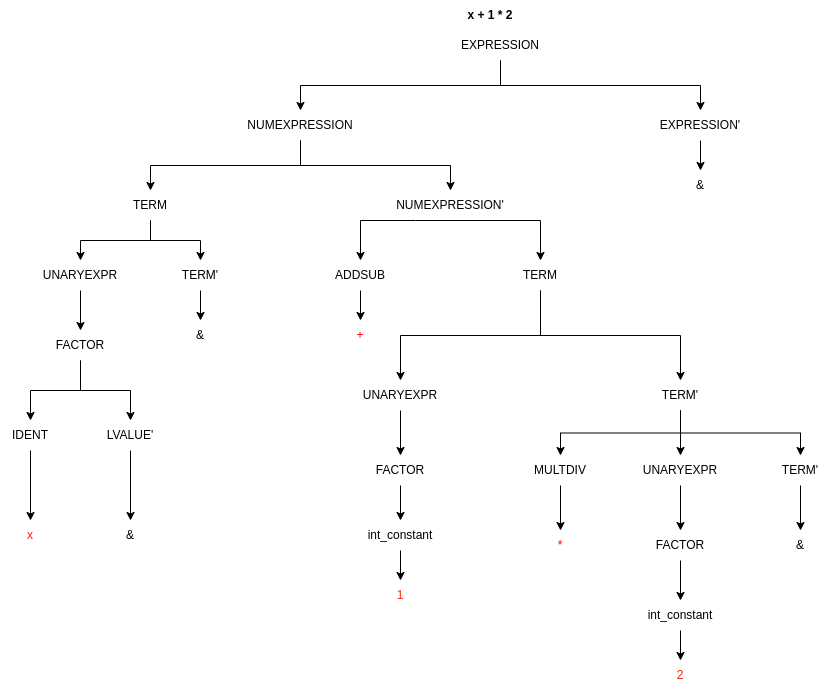
\includegraphics[scale=0.6]{tree.drawio.png}
\end{center}

\section{Inserção do tipo na tabela de símbolos}
Para realizar o processo de construção da árvore de declarações,
realizamos os mesmos procedimentos semelhantes à construção da árvore EXPA.
Primeiro, separamos a grámatica de DEC e utilizamos uma tabela de símbolos 
com uma função chamada new\_entry() para inserir na tabela. Seus parâmetros são: identificador, tipo, tabela e número da linha
em que foi encontrado.

Para demonstrar, que a SDD de DEC é L-Atribuída, basta verificar se os atributos são
sintetizados ou se são herdados pelo pai, irmão ou por si mesmo, desde que não haja ciclos entre as produções.
Ao verificar o arquivo em '\emph{Relatorio/Gramáticas/DEC.sdd}' notamos que todas produções respeitam essas condições e, portanto,
é L-Atribuída. Agora, para transformar a SDD em SDT, adicionamos as regras semânticas nas produções.
Segue abaixo uma produção chamada PARAMLIST em SDD e outra em SDT. Note que a SDT de DEC se encontra em 
'\emph{Relatorio/Gramáticas/DEC.sdt}'

\begin{python}
# PARAMLIST EM SDD

'''
paramlist : STRING listdcl IDENT paramlist1 
'''

scope = scope_stack[-1]
entry = EntradaTabela(IDENT, STRING, listdcl['dim'], [-1] * listdcl['dim'], IDENT.lineno)
scope.new_entry(entry)

paramlist = { 'dim': paramlist1['dim'] + 1, 'code': ['from_params {IDENT}', *paramlist1['code']] }    
\end{python}

\begin{python}
#PARAMLIST EM SDT

paramlist : STRING listdcl IDENT paramlist1 {
    scope = scope_stack[-1]
    entry = EntradaTabela(IDENT, STRING, listdcl['dim'], [-1] * listdcl['dim'], IDENT.lineno)
    scope.new_entry(entry)

    paramlist.dim = paramlist1['dim'] + 1
    paramlist.code = ['from_params {IDENT}', *paramlist1['code']]
}

\end{python}
\section{Verificação de Tipo}
A verificação dos tipos são necessárias para validar as entradas de uma expressão
de acordo com uma regra definida entre operações diferentes. Dentro da função
check\_type(), ela verifica o tipo dos nodos da direita e da esquerda. Caso essa combinação
não exista dentro do dicionário, é retornado o valor None e mostrado um erro chamado
\emph{InvalidTypeOperationError}, que indica um tipo de operação inválida.

\begin{python}
    
def check_type(left, right, operation, lineno):
    valids = {
        ('string', '+', 'string'): 'string',
        ('string', '+', 'int'): 'string',
        ('string', '+', 'float'): 'string',
        ('int', '+', 'string'): 'string',
        ('float', '+', 'string'): 'string',
        ('int', '+', 'int'): 'int',
        ('int', '-', 'int'): 'int',
        ('int', '*', 'int'): 'int',
        ('int', '%', 'int'): 'int',
        ('int', '/', 'int'): 'float',
        ('float', '+', 'float'): 'float',
        ('float', '-', 'float'): 'float',
        ('float', '*', 'float'): 'float',
        ('float', '/', 'float'): 'float',
        ('float', '+', 'int'): 'float',
        ('float', '-', 'int'): 'float',
        ('float', '*', 'int'): 'float',
        ('float', '/', 'int'): 'float',
        ('int', '+', 'float'): 'float',
        ('int', '-', 'float'): 'float',
        ('int', '*', 'float'): 'float',
        ('int', '/', 'float'): 'float',
    }
 
    result = valids.get((left.result_type, operation, right.result_type), None)
 
    if result is None:
        raise InvalidTypeOperationError(f'Error on operation {operation}: {left.result_type},{right.result_type},{lineno}')
 
    return result

\end{python}
\section{Verificação de Identificadores por Escopo}
A declaração de váriaveis dentro de um mesmo escopo não pode ocorrer para o mesmo
identificador com dois tipos diferentes. Por exemplo, caso a váriavel declara como int a,
não pode ser possível declarar a váriavel string a dentro do mesmo escopo.
Para tratar esse escopo, foi criado a classe Escopo e o método new\_entry().
Dentro dessa classe, foi adicionado tabela de símbolos denominada escopo, uma lista de escopo
internos e uma váriavel booleana que mostra se um escopo é um comando de repetição.
Todas as vezes que uma nova entrada é inserida, primeiro é verificado se ela já está presente na tabela.
Caso esteja presente, é retornado o
erro \emph{VariableAlreadyDeclaredError}, indicando que ela já foi declarada. 

\begin{python}
class Escopo:
    ''' Classe de Escopo '''

    def __init__(self, label='global', escopo_pai=None, loop=False):
        self.label = label
        self.escopo_pai = escopo_pai
        self.loop = loop
        self.table = []
        self.escopos_internos = []

    def new_entry(self, entry):
        '''Adiciona entrada na tabela de simbolos'''

        # Se variavel ja foi declarada
        var = list(filter(lambda x: x.ident == entry.ident, self.table))

        if len(var) > 0:
            raise VariableAlreadyDeclaredError('Variavel ja declarada')

        self.table.append(entry)
\end{python}

\section{Comandos dentro do Escopo}
A implementação da linguagem deve considerar a presença de um break fora
do escopo de um comando de repetição.

\begin{python}
def p_statement_10(p):
    '''
    statement : BREAK SEMICOLON
    '''
    scope = scope_stack[-1]
    while scope:
        if scope.loop:
            break

        scope = scope.escopo_pai

    if not scope:
        raise BreakOutLoopError(p.lineno(2))

    p[0] = { 'code': [f'goto {NEXT_LOOP_LABEL}'] }

\end{python}
Para simular o comando \emph{break} fora de um loop, é executado
o arquivo '\emph{tmp/break\_scope\_error.ccc}'.
\begin{lstlisting}[escapechar=\#]

             $ make run file='tmp/break_scope_error.ccc'

 IDENT   | (LINE,COLUMN)                                                                                       
  main   | [(1, 5)]                                                                                            
   i     | [(2, 9), (5, 9), (5, 16), (5, 24), (5, 28), (7, 13)]                                                
   a     | [(3, 9)]                                                                                            
   b     | [(4, 9), (7, 9)]                         f                                                           
Generating LALR tables
WARNING: 2 shift/reduce conflicts
Traceback (most recent call last):
  File "main.py", line 23, in <module>
    sa(input_value)
  File "/home/erik/Documents/Github/Compilador/syntax.py", line 1075,
  in analyze
    result = parser.parse(input=input_value, debug=log)
  File "/usr/local/lib/python3.8/dist-packages/ply-3.11-py3.8.egg/ply/yacc.py",
  line 329, in parse
    return self.parsedebug(input, lexer, debug, tracking, tokenfunc)
  File "/usr/local/lib/python3.8/dist-packages/ply-3.11-py3.8.egg/ply/yacc.py",
  line 503, in parsedebug
    p.callable(pslice)
  File "/home/erik/Documents/Github/Compilador/syntax.py", line 424,
  in p_statement_10

#$\textbf{raise BreakOutLoopError(p.lineno(2))}$#

classes.exception.BreakOutLoopError: 18
make: *** [Makefile:16: run] Error 1
\end{lstlisting}

\section{Geração de Código Intermediário}

Os arquivos estão em \emph{Relatorio/Gramátiocas/ConvCC-2021-1.sdd}
Os arquivos estão em \emph{Relatorio/Gramátiocas/ConvCC-2021-1.sdt}

\begin{python}
def p_forstat(p):
    '''
    forstat : new_loop_label FOR LPAREN forstat1 SEMICOLON forstat2 SEMICOLON forstat1 RPAREN new_scope_loop LBRACE statelist RBRACE
    '''
    scope_stack.pop()

    start = generate_label()
    next_label = NEXT_LOOP_LABEL

    p[0] = {
        'code': [
            *p[4]['code'],
            f'$label:{start}:',
            *p[6]['code'],
            *([f"if False {p[6]['label']} goto {next_label}"] if p[6]['label'] else []),
            *p[12]['code'],
            *p[8]['code'],
            f'goto {start}',
            f'$label:{next_label}:',
        ]
}
\end{python}
Código Intermediário

\begin{lstlisting}
    
Arquivo 'debug/ci.txt' gerado ao compilar 'lil_example.ccc'

                $ make run file='tmp/lil_example.ccc'

                     | goto L3
f:                   | 
                     | from_params a
                     | from_params b
                     | t1 = a
                     | read t1
                     | t2 = b
                     | print t2
L2:                  | 
                     | t3 = a
                     | t4 = b
                     | t5 = t3 > t4
                     | if False t5 goto L1
                     | t6 = b
                     | t7 = 2
                     | t8 = t6 - t7
                     | a = t8
                     | goto L2
L1:                  | 
                     | param t9
                     | param t10
                     | call f, 2
                     | t11 = b
                     | return t11
L3:                  | 
                     | goto L7
main:                | 
                     | from_params argn
                     | from_params argc
                     | int i
                     | t12 = 3
                     | t13 = 4
                     | int a[t12][t13]
                     | int b
                     | t14 = 0
                     | i = t14
L6:                  | 
                     | t15 = i
                     | t16 = 10
                     | t17 = t15 < t16
                     | if False t17 goto L4
                     | t21 = 2
                     | string c[t21]
                     | t22 = 0
                     | t23 = "a"
                     | c[t22] = t23
                     | t24 = 1
                     | t25 = "b"
                     | c[t24] = t25
                     | t26 = 3
                     | float b[t26]
                     | float j
                     | t27 = 3
                     | t28 = new float[t27]
                     | b = t28
                     | t29 = i
                     | print t29
                     | t30 = i
                     | t31 = 2
                     | t32 = t30 >= t31
                     | if False t32 goto L5
                     | t33 = 4
                     | j = t33
                     | goto L4
L5:                  | 
                     | t18 = i
                     | t19 = 1
                     | t20 = t18 + t19
                     | i = t20
                     | goto L6
L4:                  | 
                     | t34 = 0
                     | return t34
L7:                  | 

\end{lstlisting}
\section{Lazy Check}
Um problema encontrado no desenvolvimento do trabalho, foi a definição de funções recursivas, visto que quando uma função chama ela própria no seu código, sua definição ainda não existe na tabela de símbolos, pois essa inclusão só acontece após o final da interpretação da função. Dessa forma, para solucionar esse problema e possibilitar o uso de código recursivo, foi criada uma funcionalidade de checagem preguiçosa através da função lazy check e uma lista de variáveis que não existem no escopo. Nesse sentido, quando uma função termina de ser interpretada essa função lazy check é chamada, de forma que ela percorre essa lista de variáveis que não existem no escopo e procura pelo nome da função recursiva e caso esse nome seja encontrado, a função será reinterpretada mas agora com a definição existente na tabela de símbolos possibilitando a funcionalidade de recursão.
Segue abaixo a implementação da função lazy check.

\begin{python}
def lazy_check():
    global lazy_check_var
  
    for var in lazy_check_var:
        search_var(*var)
  
    lazy_check_var = []

def search_var(ident, line_no, lazy=False):
    global lazy_check_var
    if scope_stack:
        scope = scope_stack[-1]
        while scope:
            for e in scope.table:
                if e.ident == ident:
                    return e
            
            scope = scope.escopo_pai
        
        if lazy:
            lazy_check_var.append((ident, line_no))
            return
        else:
            raise VariableAlreadyDeclaredError(f'Linha {line_no}: Variavel {ident} nao declarada')

    raise ScopeNotExistError()
\end{python}
\section{Exceções}
\begin{python}
    class VariableAlreadyDeclaredError(Exception):
        ''' A variavel ja foi declarada '''

    class VariableNotDeclaredError(Exception):
        ''' A variavel nao foi declarada '''

    class ScopeNotExistError(Exception):
        ''' O escopo nao existe '''

    class InvalidTypeOperationError(Exception):
        ''' Tipo de operacao invalida '''

    class BreakOutLoopError(Exception):
        ''' Break fora de um loop '''

    class TypeError(Exception):
        ''' Operacao com variavel de tipo invalido '''

    class IdentifierNotFunction(Exception):
        ''' A variavel e um indentificador, nao uma funcao '''

    class ParamCountError(Exception):
        ''' Numero invalido de parametros '''
\end{python}
% ---
% Conclusão (outro exemplo de capítulo sem numeração e presente no sumário)
% ---
\chapter*[Conclusão]{Conclusão}
Os compiladores traduzem o código fonte de uma linguagem de programação
de alto nível para uma linguagem de programação de baixo nível. Sem eles 
a tarefa de programar seria um trabalho extremamente lento e difícil.
São nichos específicos e muito raros os casos em que desenvolvemos
aplicações feitas diretamente em Assembly. Nos dias atuais, quase todas linguagens
possui o seu compilador, facilitando e aumentando a efetividade dos programadores.
Dito isto, com esse trabalho, foi possível entender a primeira parte da construção
de um compilador, ou seja, do analisador léxico. Já em sua segunda parte, do analisador sintático,
compreendemos os cuidados e formas de se criar uma gramática consistente. Utilizando a ferramenta PLY,
entendemos os princípios utilizados para se construir um compilador de uma
linguagem qualquer através da sua aplicação prática. Além disso, com o Diagrama
de Transição foi possível entender como ocorre a leitura das palavras e como são
identificado os tokens. Portanto, ao realizar este trabalho,
ficou evidente como criar um compilador através de ferramentas geradores de 
analisadores léxicos e sintáticos e dos estudos e pesquisas sobre compiladores.

\addcontentsline{toc}{chapter}{Conclusão}
% ---

% ----------------------------------------------------------
% ELEMENTOS PÓS-TEXTUAIS
% ----------------------------------------------------------
\postextual
% ----------------------------------------------------------

% ----------------------------------------------------------
% Referências bibliográficas
% ----------------------------------------------------------
\bibliography{abntex2-modelo-references}

% ----------------------------------------------------------
% Glossário
% ----------------------------------------------------------
%
% Consulte o manual da classe abntex2 para orientações sobre o glossário.
%
%\glossary

%---------------------------------------------------------------------
% INDICE REMISSIVO
%---------------------------------------------------------------------
\phantompart
\printindex
%---------------------------------------------------------------------

\end{document}